%------------------------------------------------------------------
%  Document Class
%------------------------------------------------------------------
\documentclass{../class/gatech-thesis-tphmAddaptation}
%------------------------------------------------------------------
%  Graphics and Related Packages
%------------------------------------------------------------------
%\usepackage[latin1]{inputenc}
\usepackage[english]{babel}
\usepackage{amsmath}
\usepackage[dvips]{color}
\usepackage{pdflscape}
\usepackage{rotating}
\usepackage{graphicx}
\usepackage{savesym}
\savesymbol{pdfbookmark}
\usepackage{hyperref}
\restoresymbol{HR}{pdfbookmark}
%\usepackage[pdftex]{graphicx}
\graphicspath{{../../images/jpg/}}
\DeclareGraphicsExtensions{.png,.jpg}
\usepackage{url}
\usepackage{listings}
\renewcommand\figurename{Figura}
\renewcommand\chaptername{Cap\'itulo}
\renewcommand\tablename{Tabla}
\renewcommand\refname{Bibliograf\'ia}
%\renewcommand\contentsnae{Contenido} Esta generando error
\newtheorem{theorem}{Definition}[section]
%\newtheorem{definition}{\definitionname}[section]

%\usepackage{url}
%\usepackage[pdftex]{graphicx}
%\graphicspath{{../pdf/}{../../images/jpg/}{../../images/png/}}
%\DeclareGraphicsExtensions{.pdf,.jpeg,.jpg,.png}
%\usepackage{listings}
%\hyphenation{}
%\usepackage[english]{babel}
%\parskip 1ex

%------------------------------------------------------------------
%  Controls the files included for generation
%------------------------------------------------------------------
\hyphenation{op-tical net-works semi-conduc-tor cu-rrent he-te-ro-ge-neous un-ders-tood des-cri-bes go-ver-nan-ce asso-cia-ted sca-la-bi-li-ty si-mi-la-ri-ty le-vels Re-gis-tra-ti-on Re-gis-te-red owl-Func-tio-nal-Pro-per-ty owl-Ob-ject-Pro-per-ty PEN-DING}


%\includeonly {../others/dedication, ../intro/preface, ../others/acknowledgements, ../others/summary}
%------------------------------------------------------------------
%  Paper title and Author names and affiliations
%------------------------------------------------------------------

\title{KALCAS: Un frameworK para evaluaci\'on de ALineamiento de arquiteCturAS de informaci\'on y de negocio}
\author{Estudiante UFPS}
\principaladviser{Dar\'io Ernesto Correal Torres}
\firstreader{Rubby Casallas Guti\'errez}
\secondreader{Alexis Eduardo Ocampo Ramirez}
%\department{Ingenier\'ia de Sistemas y Computaci\'on}
\department{is}
\degree{Magister en Ingenier\'ia}
\copyrightyear{2012}
\bibpagetrue
\submitdate{Julio, 2012}
%------------------------------------------------------------------
%  Document
%------------------------------------------------------------------
\begin{document}
\bibliographystyle{../class/uniandes-tesis}
\bibfiles{../../bib/references}
%\bibliography{../../bib/references}

%------------------------------------------------------------------
%  Prelimary
%------------------------------------------------------------------
\begin{preliminary}
\phantomsection
\addcontentsline{toc}{chapter}{Resumen}
\chapter*{Resumen\markboth{Resumen}{}}

El alineamiento entre procesos de negocio y tecnolog\'ias de informaci\'on (IT) es la preocupaci\'on principal en los estudios de gerencia de IT, debido al impacto directo que ejerce sobre la agilidad y flexibilidad de las organizaciones. La arquitectura empresarial (EA) es un valioso instrumento para evaluar y alcanzar tal alineamiento. Los marcos de EA describen la organizaci\'on en dominios como Arquitectura de Negocio, Informaci\'on, Aplicaciones y Tecnolog\'ia. Diferentes trabajos han propuesto marcos y metodolog\'ias para evaluar la alineaci\'on a trav\'es de los elementos contenidos en los dominios de EA. Sin embargo, suponen tareas manuales como aplicar encuestas o comparar artefactos de EA. Estas tareas manuales aplicadas sobre artefactos heterog\'eneos son costosas en tiempo y recursos, propensa a errores e impr\'acticas en extensas EAs. Presentamos KALCAS, una propuesta para soportar alineamiento entre BA e IA a trav\'es de comparaci\'on autom\'atica de sus elementos constitutivos y soportado en Arquitectura Dirigida por Modelos (MDA) y Matching de Ontolog\'ias. Nuestros principales objetivos son: i) Soportar el proceso de evaluaci\'on de alineamiento entre BA e IA y ii) Automatizar la detecci\'on de potenciales alineamientos y desalineamientos  entre BA e IA. Presentamos los resultados obtenidos en la aplicaci\'on de esta aproximaci\'on en el Instituto Colombiano para la Evaluaci\'on de la Educaci\'on (ICFES).

\textit{Keywords}: Alineamiento de Negocio y Tecnolog\'ia, Detecci\'on Semi-Automatica de Trazabilidad; Heur\'isticas de Alineaci\'on, Matching de Ontolog\'ias, Modelo de EA.


%------------------------------------------------------------------
%         Abstract
%------------------------------------------------------------------
\begin{abstract}

The alignment of Business Processes and Information Technologies (IT) is among the top concerns of IT management surveys, because it has a direct impact on the organization's agility and flexibility to change in response to business needs. Enterprise Architecture (EA) is a valuable instrument to assess and achieve such alignment. EA frameworks describe the organization in domains like Business (BA), Information (IA), Application (AA) and Technology Architecture (TA). Different works have proposed frameworks and methodologies for alignment evaluation across elements contained in EA domains; however, they suppose manual tasks such as applying surveys or comparing EA's artifacts. These manual tasks applied over heterogeneous artifacts are time-costly, error-prone and impractical on large EAs. We introduce KALCAS, a framework to support the alignment between BA and IA via the automatic comparison of their constituent elements supported in Model Driven Architecture (MDA) and Ontology Matching techniques. Our key objectives are: i) To support the process of evaluating BA-IA alignment; ii) to automatically discover traceability among the elements in the BA and IA domains; iii) to detect potential alignments and misalignments between BA and IA. We present the obtained results of this approach applied in the Institute responsible for assessing the quality of education in Colombia.

\textit{Keywords}: Business-Technology Alignment, Semi-Automatic Traceability Detection; Alignment Heuristic, Ontology Matching, Enterprise Architecture Model.


\end{abstract}
\begin{dedication}
\vspace*{2in}

{\it A Dios quien, ha puesto todas las cosas importantes en mi camino, incluida esta.}

{\it A mis padres que con mucho esfuerzo lograron brindarme las bases que hoy me permiten culminar otra etapa.}

{\it A mi esposa, que ha sido el soporte sobre el cual he podido construir todo lo que me he propuesto, y que ha invertido tanto o m\'as esfuerzos que yo en la consecuci\'on de este logro.}

{\it A mi hijo Sebasti\'an, que a\'un sin saberlo, me aport\'o el sacrificio, la fuerza y la serenidad necesaria para superar las pruebas que se presentan cuando se persiguen valiosos objetivos .}


\end{dedication}
%\input{../others/preface} 
\begin{acknowledgements}

A Dios y a mi familia que han dispuesto las herramientas que hoy me permiten desarrollar esta trabajo.

Doy gracias a \textit{Dar\'io}, como asesor de tesis me brind\'o confianza para desarrollar este trabajo, por la dedicaci\'on y la gu\'ia que me permitieron encontrar la direcci\'on adecuada para llevar a buen puerto esta investigaci\'on.

Doy gracias a la \textit{Universidad de los Andes} por ayudarme a mejorar mi capacidades profesionales y desarrollarme acad\'emicamente.

Doy gracias al ICFES, a sus directivos que facilitaron el desarrollo de mi maestr\'ia, y al valioso grupo de colegas que generosamente me apoyaron en el proceso de validaci\'on de esta propuesta.

Finalmente, a los amigos que me brindaron su apoyo y aliento en momentos complicados durante el desarrollo de toda mi maestr\'ia.

\end{acknowledgements}
\contents
%\input{../others/summary}
\end{preliminary}

%------------------------------------------------------------------
%         Chapters
%------------------------------------------------------------------
%=================================================================
\chapter{INTRODUCCI\'ON} \label{cha:intro}
%=================================================================

La alineaci\'on entre negocio y tecnolog\'ia puede ser definida como la forma de cuantificar el nivel de coherencia entre las necesidades del negocio y la respuesta ofrecida por las Tecnolog\'ias de Informaci\'on (IT) \cite{Pereira:2003}. Esta alineaci\'on es un tema clave en todas las organizaciones. Cada a\~no, cuando los directores de tecnolog\'ia son encuestados para identificar sus principales prioridades, la necesidad de alinear negocio y IT aparece en los primeros lugares \cite{Wang:20082}. Gestionar y evaluar la alineaci\'on negocio-IT no es f\'acil, ni en su conceptualizaci\'on ni en su realizaci\'on \cite{Scott:2005}. La falta de alineaci\'on es una de las razones fundamentales por la cual las empresas no pueden alcanzar todo el potencial de sus inversiones en IT \cite{Cuenca:2010}. Informaci\'on desactualizada, procesos repetitivos no automatizados, silos de informaci\'on, procesos y entidades redundantes son ejemplos comunes de dicha desalineaci\'on. 

Estudios anteriores \cite{henderson:1990, Bergeron:2004, Elhari:2011, Plazaola:2008, Wang:2008} han propuesto marcos te\'oricos y metodolog\'ias de alineaci\'on centrados en la aplicaci\'on de encuestas sobre la percepci\'on y tabulaci\'on de resultados; pero en general no abordan un an\'alisis apoyado en herramientas automatizadas. 

La Arquitectura Empresarial (EA) se presenta como un elemento importante para alcanzar la alineaci\'on negocio-IT \cite{Lankhorst:2004}. Una EA describe la organizaci\'on en dimensiones o arquitecturas como Negocio (BA), Informaci\'on (IA), Aplicaciones (AA) y Tecnolog\'ia (TA) y se han propuesto frameworks para evaluaci\'on del alineamiento a trav\'es de los elementos contenidos en estos dominios.

Varias propuestas \cite{Pereira:2003, Pereira:2005, Sousa:2005, Wegmann:2005, Cuenca:2010} abordan el alineamiento desde la perspectiva de la correspondencia entre los elementos o componentes de los dominios de EA ( i.e. BA, IA, AA y TA). Para determinar esta correspondencia se requiere identificar los diferentes elementos de la EA, compararlos, establecer las relaciones o trazas entre las diferentes dimensiones y evaluarlos aplicando reglas heur\'isticas \cite{Pereira:2003, Pereira:2005, Sousa:2005} que detectan s\'intomas de potenciales desalineaciones. Algunas de las heur\'isticas de alineaci\'on BA-IA propuestas son: i) Redundancia de procesos de negocio y activos de informaci\'on, ii) procesos que no acceden a ninguna entidad y iii) entidades que no son accedidas por ning\'un proceso.

Seg\'un \cite{wegmann:2003, Wegmann:2005, Anaya:2005}, dado que uno de los prop\'ositos de la EA es alinear negocio e IT, el concepto de \textit{trazabilidad} es esencial para hacer expl\'icita la manera como esta integraci\'on es alcanzada en todos los niveles organizacionales. Por tanto \cite{wegmann:2003} define la trazabilidad como la capacidad para hacer expl\'icitas las relaciones entre elementos que se encuentran en diferentes niveles de la EA y que refleja un nivel de alineaci\'on e integraci\'on entre ellos.

Nuestra aproximaci\'on est\'a en l\'inea con los trabajos previos y entiende la trazabilidad como un s\'intoma o indicador de alineaci\'on de Negocio-IT que puede ser inferido partir de los elementos contenidos en una EA. Estudios anteriores sobre evaluaci\'on de alineaci\'on Negocio-IT a trav\'es de los artefactos de EA coinciden en un conjunto de tareas necesarias para implementar tal evaluaci\'on: i) Identificar los elementos de cada dimensi\'on de la EA, ii) comparar los elementos de cada dimensi\'on de la EA, iii) definir relaciones entre estos elementos (trazabilidad), iv) identificar alineaciones y desalineaciones y v) asignar un nivel de alineaci\'on.

%=================================================================
\section{Planteamiento del Problema} \label{sec:problem}
%=================================================================

A pesar que uno de los principales objetivos de los marcos de EA es proveer representaciones integradas entre los diferentes niveles organizacionales, es dif\'icil establecer claramente la trazabilidad entre ellos \cite{wegmann:2003}. La verificaci\'on de la alineaci\'on y la trazabilidad con el paradigma de modelado por dimensiones se ha convertido en un problema importante \cite{Wegmann:2005}. 

Hasta donde conocemos, algunas tareas involucradas en la evaluaci\'on de alineamiento como: Comparar los elementos de EA e identificar trazabilidad entre elementos de diferentes niveles se realizan tradicionalmente de forma manual. Esto implica revisar y comparar manualmente un conjunto de artefactos heterog\'eneos (diagramas, documentos de texto, hojas de c\'alculo, im\'agenes) que describen una EA. Entre m\'as elementos tiene cada dominio de EA, m\'as complejo es el concepto y la evaluaci\'on del alineamiento, porque m\'as reglas y heur\'isticas necesitan ser definidas y aplicadas para gobernar las relaciones entre dichos elementos \cite{Sousa:2005}. Un procedimiento manual de revisi\'on, comparaci\'on y asociaci\'on implica una alta probabilidad de error, gran inversi\'on de tiempo y recursos \cite{Rahm:2001}. El problema se profundiza en grandes organizaciones con complejas y extensas EA que contienen cientos de artefactos, por lo que esta tarea no solo es compleja, sino a veces inviable en la pr\'actica. 

La preguntas de investigaci\'on que abordamos en este trabajo son: 
\begin{itemize}
\item \textbf{RQ1:} ?`Es posible automatizar tareas de evaluaci\'on de alineaci\'on entre BA-IA y de que manera?
\item \textbf{RQ2:} ?`Existe un beneficio en t\'erminos de precisi\'on y agilidad al apoyar las tareas de evaluaci\'on de alineaci\'on entre BA-IA con una aproximaci\'on automatizada orientada por modelos y matching de ontolog\'ias?
\end{itemize}

%===============================================================
\section{Objetivos y Contribuciones} \label{subsec:objective}
%===============================================================

Los principales objetivos de nuestra propuesta son: i) Apoyar el proceso de evaluaci\'on de alineaci\'on entre BA-IA. ii) Descubrir autom\'aticamente trazabilidad entre elementos de los dominios de BA e IA. iii) Detectar alineaciones y desalineaciones potenciales entre BA-IA en el marco de una EA.

Las contribuciones centrales de este trabajo se resumen as\'i: Extendemos un metamodelo de EA para formalizar las asociaciones BA-IA. Definimos un procedimiento para inferir trazabilidad entre elementos de BA e IA, apoyado en matching de Ontolog\'ias. Construimos Kalcas Query Language (KQL), un Domain Specific Language (DSL) gr\'afico que permite realizar consultas de alineaciones y desalineaciones entre BA-IA consignadas en el modelo de EA.

%===============================================================
\section{Estructura del Documento} \label{subsec:structure}
%===============================================================
El resto de este documento esta organizado de la siguiente manera: El Cap\'itulo \ref{cha:background} describe el contexto asociado a la problem\'atica y en el cual podemos basar nuestra estrategia. El Cap\'itulo \ref{cha:studycase} ofrece un caso de estudio para motivar nuestra aproximaci\'on. En el Cap\'itulo \ref{cha:solution} presentamos nuestra propuesta de soluci\'on. El lenguaje de consulta KQL es detallado en el Cap\'itulo \ref{cha:KQL}. El Cap\'itulo \ref{cha:implementacion} ofrece en detalle la implementaci\'on de esta propuesta. La experimentaci\'on y evaluaci\'on realizada se expone en el Cap\'itulo \ref{cha:evaluation}. El  Cap\'itulo \ref{cha:relatedwork} describe el trabajo relacionado. Y finalmente el Cap\'itulo \ref{cha:conclusions} reporta las conclusiones y el trabajo futuro.
%=================================================================
\chapter{CONTEXTO} \label{cha:background}
%=================================================================

En este cap\'itulo se realiza una revisi\'on de los conceptos empleados durante el desarrollo de este documento. 

%**************************************************************
\section{Alineaci\'on de Negocio-IT} \label{sec:bitalignment}
%**************************************************************
La alineaci\'on entre negocio y tecnolog\'ia puede ser definida como la forma de cuantificar el nivel de coherencia entre las necesidades del negocio y la respuesta ofrecida por las Tecnolog\'ias de Informaci\'on (IT) \cite{Pereira:2003}. Henderson y Venkatraman \cite{henderson:1990} definen el alineamiento estrat\'egico a partir de cuatro componentes: i) Estrateg\'ia de Negocio, ii) estrateg\'ia de IT, iii) procesos e infraestructura organizacional, y iv) procesos e infraestructura de IT. Las diferentes relaciones que se dan entre estos componentes son definidas como \textit{Alineamiento Estrat\'egico}, \textit{Alineamiento Funcional} y \textit{Alineamiento Transversal}.

Otros trabajos \cite{Pereira:2005, Wang:2008, Wang:20082, Plazaola:2008} han abordado la gesti\'on y evaluaci\'on del alineamiento en t\'erminos de los componentes contenidos en la EA. En la misma l\'inea, para el framework SEAM \cite{Wegmann:2005} el alineamiento negocio-IT corresponde a la trazabilidad entre los niveles de negocio, operaci\'on e IT. 

%**************************************************************
\section{Arquitectura Empresarial} \label{sec:eamda}
%**************************************************************

Una Arquitectura Empresarial (EA) ofrece la descripci\'on integral y estructurada de la organizaci\'on, sus Sistemas de Informaci\'on (IS), y la forma en que estos se integran a fin de alcanzar los objetivos de negocio apoyados en Tecnolog\'ias de Informaci\'on (IT). Esta descripci\'on se compone de documentos, diagramas y dem\'as artefactos que formalizan diferentes puntos de vista de la organizaci\'on, de tal manera que sean un referente y soporte para la toma de decisiones. Los frameworks tradicionales de EA como \cite{Zachman:1987, DoDAF:2005, OpenGroup:2008}, tienen en com\'un la desagregaci\'on en dimensiones: i) La \textit{Arquitectura de Negocio} (BA) define la estrategia, gobernabilidad, organizaci\'on y procesos claves de negocio. ii) La \textit{Arquitectura de Datos} (IA) describe la estructura de los activos de datos l\'ogicos y f\'isicos de la organizaci\'on y los recursos de gesti\'on de datos. iii) La \textit{Arquitectura de Aplicaciones} provee un modelo para las aplicaciones a ser desplegadas, sus interacciones y sus relaciones con los principales procesos de negocio de la organizaci\'on. iv) En la \textit{Arquitectura de Tecnolog\'ia} se describen las capacidades de software y hardware que son requeridas para el despliegue de servicios de negocio, datos y aplicaciones.

%===============================================================
\section{Arquitectura Dirigida por Modelos} \label{subsec:mda}
%===============================================================

Model-Driven Architecture (MDA) es una propuesta de la OMG para abordar el desarrollo de software proporcionando un conjunto de gu\'ias para estructurar especificaciones expresadas en modelos. Es neutral en cuanto a tecnolog\'ia y proveedor, y busca reducir significativamente el esfuerzo de desarrollo, separando la arquitectura del sistema, de las arquitecturas de plataforma. Uno de los elementos claves de MDA es el Modelo de Plataforma Independiente (\textit{PIM}) que describe la estructura y el comportamiento de un sistema, pero no su implementaci\'on. La implementanci\'on en la plataforma particular (JEE, .NET, WS, etc) est\'a definida en un Modelo de Plataforma Espec\'ifica (\textit{PSM}), el cual es originado a partir del PIM. Para materializar esta conversi\'on, se realizan transformaciones basadas en plantillas detalladas para cada plataforma, que mapean elementos del PIM hacia elementos PSM.

%===============================================================
\section{Tartarus} \label{subsec:tartarus}
%===============================================================


Tartarus es un acercamiento MDA para el an\'alisis de EAs \cite{Moosas:2011}. Tartarus surge como una opci\'on de soluci\'on ante la actual variedad de frameworks, est\'andares, herramientas y formatos que hacen parte de la definci\'on de una EA \cite{Rodriguez:2011}. El metamodelo descrito en la Figura \ref{fig:Tartarus-MM} est\'a compuesto por cinco paquetes: \textit{Enterprise} contiene la estructura, cadena de valor, principios, incentivos organizacionales y dem\'as elementos estrat\'egicos. \textit{Continuum} re\'une las definiciones para describir la manera en que la EA evoluciona. \textit{Management} tiene los factores necesarios para evaluar los artefactos que conforman una arquitectura. \textit{Environment} comprende el conjunto de elementos que describen el entorno en el que funciona la empresa. 

%........................................................
\begin{figure}[!t]
\begin{center}
	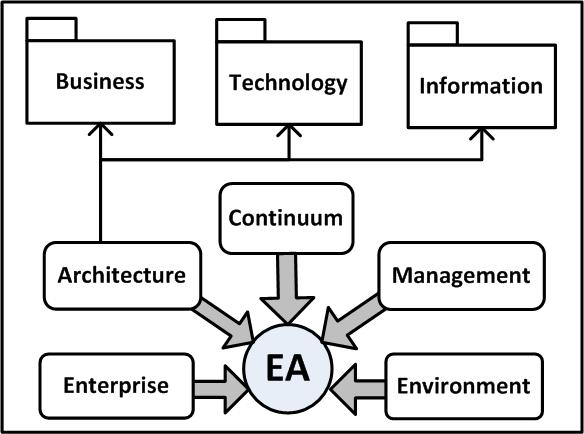
\includegraphics[scale=0.8 ,natwidth=584pt, natheight=434pt]{TartarusMM.jpg}
	\caption{Vista General del Metamodelo Tartarus}
	\label{fig:Tartarus-MM}
\end{center}
\end{figure}
%........................................................

\textit{Architecture} agrupa los conceptos clave para visualizar y estructurar la EA. \textit{Architecture} contiene los cuatro dominios: \textit{Business Domain}: Describe los procesos de negocio. \textit{Technology Domain}: Comprende las capacidades de software y hardware que soportan los servicios de negocio e informaci\'on. \textit{Information Domain}: Estructura los componentes de datos que conforman la informaci\'on de la empresa.

Vamos a describir el metamodelo, detallando el dominio de informaci\'on (izquierda), procesos de negocio (derecha) como parte del contexto de nuestro trabajo. La Figura \ref{fig:BA-IA-MM} muestra el metamodelo de los dominios mencionados.

%........................................................
\begin{landscape}

\begin{figure}[!t]
\begin{center}
	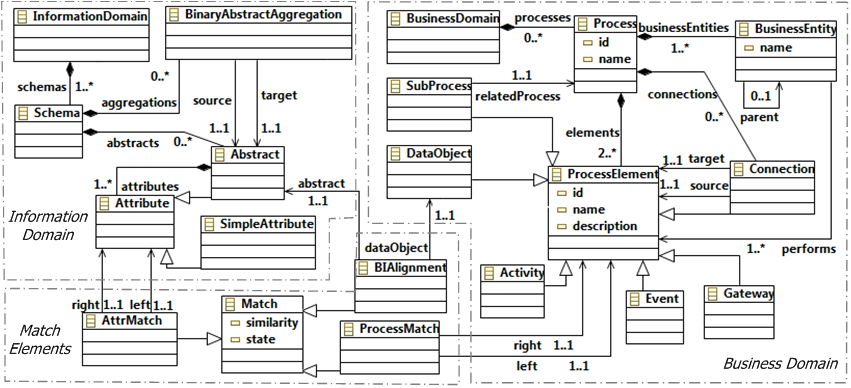
\includegraphics[scale=1 ,natwidth=851pt, natheight=388pt]{IA-BA_MM.png}
	\caption{Detalle del Metamodelo Tartarus y las Extensions  Kalcas}
	\label{fig:BA-IA-MM}
\end{center}
\end{figure}

\end{landscape}
%........................................................


%===============================================================
\subsection{Arquitectura de Negocio (BA)}
%===============================================================

Este dominio define los procesos de negocio de la compa\~n\'ia. En el metamodelo se resaltan los elementos de proceso (\texttt{ProcessElements}), Entidades de Negocio, Objetos de Flujo y Conexiones. El metamodelo aborda los diferentes tipos de actividades, eventos y flujos derivados de la nomenclatura BPMN (Business Process Modeling Notation). El concepto \texttt{DataObject} asocia las entidades de datos le\'idas y/o producidas por las actividades.

Para nuestro caso el Proceso de Registro corresponde a un elemento \texttt{Process} el cual contiene las once actividades (\texttt{Activity}) conectadas por elementos de clase \texttt{Connection} y/o \texttt{Gateway}. Los objetos de datos como \texttt{Payment Format} y \texttt{Card} se consignan como instancias de tipo \texttt{DataObject}.


%===============================================================
\subsection{Arquitectura de Informaci\'on (IA)}
%===============================================================

Nuestro metamodelo de arquitectura de informaci\'on es una adaptaci\'on del trabajo propuesto en \cite{Atzeni:2008}, enriquecido con las definiciones de las relaciones inferidas entre entidades, comentarios de tablas y comentarios de columnas. La metaclase \texttt{Schema} representa los esquemas contenidos en la EA. Para nuestro caso, el esquema \texttt{S1} se convierte en la instancia \texttt{Schema:S1}. La metaclase \texttt{Attribute} est\'a especializada en dos subclases: \texttt{SimpleAttribute} la cual define columnas en la base de datos o tipos primitivos en esquemas XML, tienen un tipo de dato (\texttt{INTEGER, DOUBLE, STRING}, etc). Por otro lado, \texttt{Abstract} se refiere a entidades en un modelo relacional o tipos de dato complejos en XML Schema.

Por ejemplo, la entidad \texttt{USER} del esquema \texttt{S1} se convierte en un objeto \texttt{Abstract:S1.USER} y cada uno de sus campos (\texttt{name, document}, etc) son objetos de clase \texttt{SimpleAttribute} con sus respectivos tipos de dato. En \texttt{BinaryAbstractAggregation}, se definen las relaciones existentes entre cada par de elementos \texttt{Abstract}. La relaci\'on entre las entidades \texttt{USER} e \texttt{REGISTRATION} se representa con la asociaci\'on \texttt{BinaryAbstractAggregation: USER\_REGISTRATION}. 


%===============================================================
\section{Ontolog\'ias} \label{subsec:ontology}
%===============================================================

Una ontolog\'ia, b\'asicamente, es una descripci\'on expl\'icita de un dominio de conocimiento espec\'ifico, definida en t\'erminos de sus conceptos, propiedades, atributos, restricciones e individuos \cite{Noy:2001}. Formalmente podemos definir una ontolog\'ia como: $O = \lbrace C, P, H^{C}, H^{P}, A^{O}, I, R^{I} \rbrace$. Donde $C$ es el conjunto de conceptos, $P$ el conjunto de propiedades. $H^{C}$ es la jerarqu\'ia de relaciones entre los conceptos tal que $H^{C} \subset C \times C (c_{i},c_{j}) \in H^{C}$ denota que el concepto $c_{i}$ es subconcepto de $c_{j}$. De la misma manera $H^{P}$ define las relaciones jer\'arquicas entre propiedades. $A^{O}$ es el conjunto de axiomas. I comprende el conjunto de Individuos, es decir, instancias de conceptos y propiedades quienes se asocian a trav\'es de instancias relacionales $R^{I}$. Una de las principales ventajas de las ontolog\'ias, es proveer caracter\'isticas \'utiles para sistemas inteligentes, representaci\'on e ingenier\'ia de conocimiento \cite{Gasevic:2009}.

%===============================================================
\subsection{Matching de Ontolog\'ias} \label{subsec:matching}
%===============================================================

La funci\'on de alineaci\'on de ontolo\'ias ha sido definida formalmente \cite{Euzenat:2007, Gal:2009}: $f(O_{1},O_{2}) = \lbrace e_{i1}, e_{i2}, i_{i}, r_{i}\rbrace$. Donde $O_{1}$ y $O_{2}$ son los esquemas/ontolog\'ias de entrada, com\'unmente llamados origen y destino respectivamente, $e_{i1}$ y $e_{i2}$ son las dos entidades comparadas, $i_{i}$ corresponde al \'indice de similitud o confianza (medido entre 0 y 1) y $r_{i}$ la relaci\'on (igualdad, especializaci\'on, generalizaci\'on) que puede haber entre $e_{i1}$ y $e_{i2}$. Detectar elementos similares entre diferentes fuentes de informaci\'on es tambi\'en una necesidad central en procesos de evaluaci\'on, migraci\'on, integraci\'on y evoluci\'on de SI, intercambio de informaci\'on en sistemas P2P y composici\'on de web services \cite{Euzenat:2007}.

En 2004 surge la Ontology Alignment Evaluation Initiative (\textit{OAEI}), una iniciativa que anualmente eval\'ua sistemas de alineamiento de ontolog\'ias. El objetivo de la OAEI es comparar diferentes propuestas, con el objetivo de ofrecer conclusiones sobre las mejores t\'ecnicas y estrategias, para lo cual, provee unos casos de prueba sobre los cuales los diferentes sistemas experimentan.  Entre los temas evaluados se encuentran: \textit{The benchmark track, The directories and thesauri track, Instance matching}. 

Existen diferentes m\'etodos y t\'ecnicas para implementar alineamiento autom\'atico de ontolog\'ias \cite{Madhavan:2001, Rahm:2001, Shvaiko:2005} y nuestra propuesta incluye algunos de ellos. Las principales t\'ecnicas de alineamiento son \textit{basadas en esquema}, \textit{basadas en contenido} y \textit{combinadas}. Las \textit{basadas en esquema} s\'olo tienen en cuenta la informaci\'on estructural del esquema, no su contenido. Dentro de este grupo se aplican comparaciones ling\"u\'isticas, textuales, de restricciones y estructurales. Las estrategias \textit{basadas en contenido} involucran estad\'isticas, patrones o incluso los mismos datos para inferir correspondencias. Las t\'ecnicas \textit{combinadas} aplican, en conjunto, las anteriores aproximaciones en busca de mejores resultados. Esta combinaci\'on puede ser configurada manual o autom\'aticamente utilizando aprendizaje de m\'aquina. 

Este trabajo no busca determinar la mejor forma de realizar alineamientos, sino adaptar y aplicar t\'ecnicas y avances en el \'area de matching de ontolog\'ias para inferir trazabilidad entre componentes de procesos e informaci\'on.
%=================================================================
\chapter{SINZA} \label{cha:conclusions}
%=================================================================

En este cap\'itulo discutimos SOBRE SINZA%**************************************************************
\section{Trabajo Futuro} \label{sec:futurework}
%**************************************************************

Las siguientes son algunas propuestas de trabajo futuro que hemos visualizado como continuaci\'on o extensiones a nuestra propuesta:

\begin{itemize}

\item Futuras investigaciones pueden incorporar la definici\'on de m\'etricas de alineaci\'on que permitan evaluar una EA frente a niveles de madurez presentados en trabajos anteriores como \cite{Elhari:2011}.

\item La inclusi\'on de los dem\'as dominios de la EA como Aplicaciones (AA) y Tecnolog\'ia (TA) mejorar\'ia la completitud de esta propuesta. Inferir trazabilidad con elementos que hacen parte de la estrategia de la organizaci\'on como drivers, principios, objetivos aportar\'ia acercar\'ia mas nuestra propuesta a la alineaci\'on negocio-IT. En este punto hay consideraciones importantes a investigar, como el hecho de alinear elementos a diferente nivel de granularidad, como lo son por ejemplo un driver de negocio y una entidad de informaci\'on.

\item Los mapeos generados con este framework podr\'ian exportarse a lenguajes est\'andar de integraci\'on de EA como ArchiMate \cite{Jonkers:2004}. De tal manera que diferentes herramientas puedan reutilizar las inferencias alcanzadas con Kalcas. Otros tipos de consultas que resuelvan diferentes preguntas sobre el modelo pueden enriquecer el editor KQL, por ejemplo obtener todas las actividades o entidades que no est\'en alineadas.

\item Las tareas de alineamiento en la fase de experimentaci\'on han utilizado algunos algoritmos de Alignment API, extender las pruebas en cuanto a motores y algoritmos para evaluar mas resultados puede mejorar la exactitud promedio de Kalcas. Para el momento de nuestro trabajo no hay disponible un algoritmo ling\"u\'istico aplicable al idioma espa\~nol, por tanto un avance en esa direcci\'on es muy valioso no solo para esta propuesta sino para el campo del matching de ontolog\'ias en general. 

\item En este trabajo se utiliz\'o la trazabilidad inferida para apoyar an\'alisis de alineaci\'on, pero nuevas investigaciones pueden emplear la trazabilidad para soportar el an\'alisis de impacto en una EA. Nuestra propuesta podr\'ia ser extendida o modificada para ser usada con otros metamodelos de EA diferentes a Tartarus.

\end{itemize}

%**************************************************************
\section{Publicaciones} \label{sec:publish}
%**************************************************************
Durante toda la realizaci\'on de este trabajo de tesis, fueron aceptadas publicaciones en modalidad \textit{full research papers} en los siguientes eventos internacionales:

\begin{itemize}

\item 16th East-European Conference on Advances in Databases and Information Systems
(ADBIS 2012): KALCAS: A frameworK for semi-Automatic aLignment of data and business proCesses ArchitectureS. Poznan, Polonia. Septiembre 2012.

\item XXX International Conference of the Chilean Computer Science Society (SCCC 2011): An Ontology-Matching based Proposal to Detect Potential Redundancies on Enterprise Architectures. Curic\'o, Chile. Noviembre 2011.

\item XXXVII Conferencia Latinoamericana de Inform\'atica (XXXVII CLEI): Detecci\'on de Elementos Redundantes en
Arquitecturas de Informaci\'on: Un Enfoque Apoyado en Alineaci\'on de Ontolog\'ias. Quito, Ecuador. Octubre 2011.

\end{itemize}



%%=================================================================
\chapter{AUTO-ADAPTABILIDAD} \label{cha:elementos}
%=================================================================


%%**************************************************************
\chapter{KALCAS: Un frameworK para evaluaci\'on de ALineamiento de arquiteCturAS de informaci\'on y procesos de negocio} \label{cha:solution}
%**************************************************************

%===============================================================
\section{Conceptualizaci\'on} \label{sec:conceptualization}
%===============================================================
Definimos formalmente los conceptos de alineaci\'on y redundancia en t\'erminos de los elementos de BA e IA con el objetivo de automatizar la tareas de comparar los elementos de cada dimensi\'on e inferir trazabilidad, las cuales fueron abordadas en el Cap\'itulo \ref{cha:intro}. Para el prop \'osito de este trabajo, asumimos la trazabilidad como un s\'intoma de alineaci\'on y la redundancia como una se\~nal de potencial desalineamiento.

El problema de identificaci\'on de trazabilidad BA-IA, podemos formalizarlo como una funci\'on entre los conjuntos de componentes que conforman estas arquitecturas.

\begin{theorem}
\label{def:traceability}
Sea ($C_{i}$) un componente de negocio, definimos que presenta trazabilidad con un componente de Informaci\'on ($C_{j}$) si tiene una correspondencia superior a un umbral de similitud ($TH$):
\begin{center}
\begin{math}
traceability(C_{i},C_{j}) \Longrightarrow C_{i} \in BA \wedge C_{j} \in IA \wedge sim(C_{i},C_{j}) \geq\ TH
\end{math}
\end{center}
\end{theorem}

Por otro lado, la definici\'on de redundancia dentro de los elementos de cada dominio, la entendemos como la relaci\'on de semejanza entre componentes del mismo dominio.

\begin{theorem}
\label{def:redundancy}
Sean ($C_{i}$ y $C_{j}$) componentes dentro del mismo dominio de EA cuyo \'indice de similitud superior a un umbral dado ($TH$): 
\begin{center}
\begin{math}
redundancy(C_{i},C_{j}) \Longrightarrow (C_{i}, C_{j} \in BA \vee C_{i}, C_{j} \in IA ) \wedge sim(C_{i},C_{j}) \geq\ TH
\end{math}
\end{center}
\end{theorem}

Estas definiciones nos permiten calcular que: El total de comparaciones de alineaci\'on est\'a dado por el producto cartesiano ($M \times N$), donde $M$ es la cantidad de elementos de $BA$ y $N$ la cantidad de elementos de $IA$. La cantidad de verificaciones de redundancia est\'a dada por el coeficiente binomial $\frac{{n!}}{2!(n-2)!}$, donde $n$ es la cantidad de elementos a contrastar en cada dominio ($M$ o $N$). De lo anterior se concluye que el orden de complejidad algor\'itmico de la funci\'on $traceability$ es de la forma $O(m \times n)\simeq O(n^2)$. El orden de complejidad de la funci\'on $redundancy$ es de la forma $O(\frac{n^2}{2}) \simeq O(n^2)$. Por tanto las dos funciones tienen un orden de complejidad cuadr\'atico lo que nos permite decir que son \textit{abordables} desde el punto de vista computacional.

Con las definiciones de \textit{traceability} y \textit{redundancy} podemos ahora proponer nuestra definici\'on de alineaci\'on entre BA-IA:

\begin{theorem}

\label{def:alignment}
Sea ($C_{i}$) un componente de negocio o Informaci\'on, definimos que est\'a potencialmente alineado si presenta trazabilidad con  elementos de otro dominio y no incurre en redundancia con elementos del dominio:
\begin{center}
\begin{math}
alignment(C_{i}) \Longrightarrow C_{i} \in traceability(C_{i},C_{j}) \wedge C_{i} \notin redundancy(C_{i},C_{j})
\end{math}
\end{center}
\end{theorem}


%===============================================================
\section{Extensiones al metamodelo Tartarus}
%===============================================================

Como parte de nuestro trabajo, extendimos el metamodelo de procesos de negocio e informaci\'on, con el prop\'osito de expresar las correlaciones que se pueden dar entre los diferentes elementos. Los \textit{Match Elements} se pueden observar en la parte inferior de la Figura \ref{fig:BA-IA-MM} y las relaciones de estas metaclases con las funciones de trazabilidad y redundancia se detallan en la Figura \ref{fig:Aling_Redund_mm}.

%........................................................


\begin{figure} [!t]
\begin{center}
	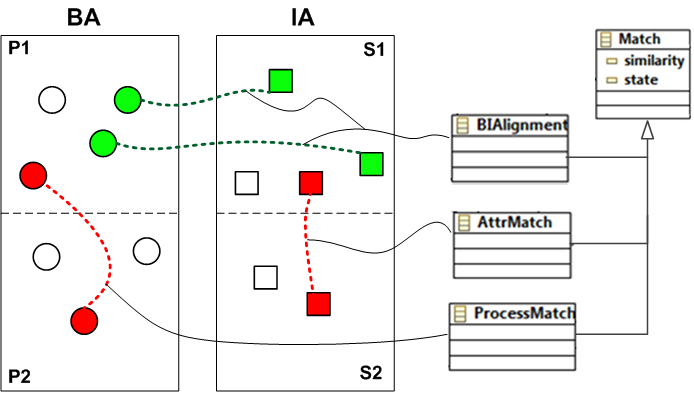
\includegraphics[scale=0.45,natwidth=694pt, natheight=398pt]{Aling_Redund_mm.png}
	\caption{Expresi\'on de Trazabilidad y Redundancia sobre las Extensiones del Metamodelo Tartarus}
	\label{fig:Aling_Redund_mm}
\end{center}
\end{figure}
%........................................................

La superclase \textit{Match} representa las correspondencias tanto de componentes dentro el mismo dominio (posibles redundancias) como de dominios diferentes (posibles alineaciones) asignando un \'indice de similitud y el estado de revisi\'on (\textit{PENDING} o \textit{VERIFIED}). Esta clase se especializa en cada tipo de mapeo: \textit{AttrMatch} asocia pares de \textit{Attribute} de diferentes esquemas, por ejemplo, una coincidencia entre la entidad \textit{S1.REGISTRATION} y \textit{S2.REGISTERED}. De una manera an\'aloga \textit{ProcessMatch} representa coincidencias potenciales entre pares de \textit{ProcessElement} por ejemplo, entre las actividades \textit{P1.Register} y \textit{P2.Migrate Registration}. Finalmente, la subclase \textit{BIAlignment} permite vincular los dominios de Informaci\'on y Negocio (alineamiento BA-IA) mediante la asociaci\'on directa entre objetos \textit{Abstract} y \textit{DataObject}.


%===============================================================
\section{Estrategia}
%===============================================================

El n\'ucleo de nuestra aproximaci\'on es el modelo Tartarus de la organizaci\'on, donde est\'an expresados formalmente los componentes de la EA, es decir los conjunto de IA y BA. El objetivo central es definir los conjuntos de BA e IA y aplicar las funciones de alineaci\'on y redundancia utilizando un motor de alineamiento de ontolog\'ias para inferir \'indices de similitud entre los elementos de ambos conjuntos.

Nuestra estrategia para inferir trazabilidad y detectar desalineaciones consta de cinco fases, cada una de las cuales es soportada por herramientas construidas dentro de este trabajo. El usuario participa verificando los mapeos candidatos inferidos autom\'aticamente por el motor de matching (de all\'i que nuestra aproximaci\'on es semi-autom\'atica) y realizando consultas de alineamiento sobre el modelo utilizando nuestro DSL gr\'afico KQL que se detallar\'a en el Cap\'itulo \ref{cha:KQL}. Una vista general de nuestra propuesta de soluci\'on se muestra en la Figura \ref{fig:Solution}.

%........................................................
\begin{figure} [!t]
\begin{center}
	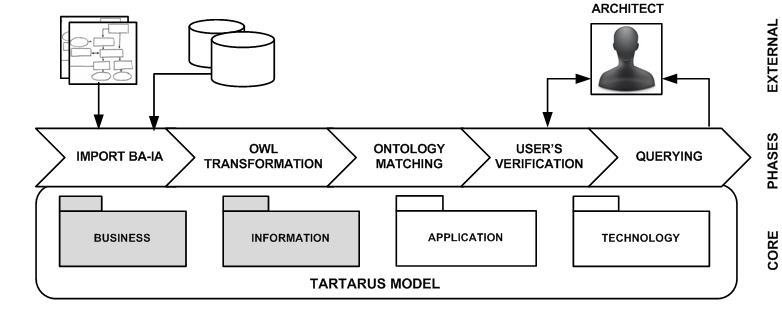
\includegraphics[scale=0.7,natwidth=782pt, natheight=309pt]{Solution_Overview2.png}
	\caption{Vista General de la Soluci\'on}
	\label{fig:Solution}
\end{center}
\end{figure}
%........................................................


%===============================================================
\subsection{Importar arquitecturas de negocio e informaci\'on}
%===============================================================

Inicialmente se requiere identificar los elementos de cada dimension de la EA, para tal fin, se importan mediante una herramienta que puebla el modelo, desde un archivo XML Process Definition Language (XPDL) para la BA o v\'ia JDBC (base de datos relacional) para la IA. Los archivos XPDL son importados mediante un \textit{serializer} desarrollado en \cite{Rodriguez:2011} el cual utiliza la librer\'ia \textit{XStream} que serializa objetos a XML y viceversa. A la versi\'on preliminar se agregaron conversores de \textit{Data Objects}, elementos necesarios en la inferencia de los alineamientos en nuestra propuesta. Los esquemas se acceden a trav\'es de una conexi\'on JDBC. Se obtiene la metadata utilizando las facilidades ofrecidas dentro del paquete \textit{java.sql}. 

En esta fase, tanto los elementos de cada conjunto, como sus estructuras y la metadata asociada son incorporados en las descripciones formales, a fin de obtener modelos enriquecidos que favorezcan las inferencias. El modelo Tartarus es creado y poblado program\'aticamente utilizando a trav\'es de las librer\'ias java que ofrece Eclipse Modeling Framework (EMF). Para el caso del ICFES, se obtiene el modelo \textit{ICFES.tartarus} expresado en conceptos Tartarus y una vista de los principales elementos del modelo se muestran en la Figura \ref{fig:icfesmodel}. 

%........................................................
\begin{figure} [!t]
\begin{center}
	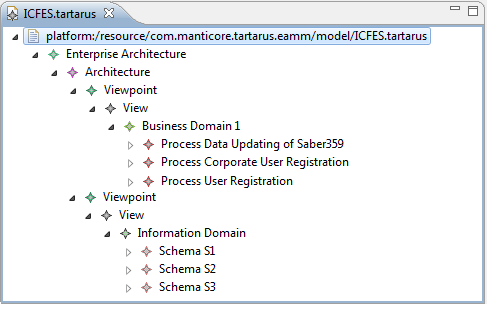
\includegraphics[scale=0.75,natwidth=487pt, natheight=307pt]{ICFEStartarus.png}
	\caption{EA del ICFES Importada al modelo Tartarus}
	\label{fig:icfesmodel}
\end{center}
\end{figure}
%........................................................

%===============================================================
\subsection{Transformaciones OWL}
%===============================================================
Posteriormente, se ejecuta una transformaci\'on Xpand \cite{Xpand:2006}, para para llevar todas las definiciones consignadas en el modelo Tartarus a ontolog\'ias OWL. Se genera un archivo OWL por cada esquema y proceso contenido en el modelo Tartarus. Para el caso del modelo \textit{ICFES.tartarus}, se generan cuatro ontolog\'ias: \textit{S2.owl}, \textit{S1.owl}, \textit{User Registration.owl} y \textit{Corporate User Registration.owl}.

La Tabla \ref{tab:tartarusowl} resume las correspondencias entre las clases Tartarus y los elementos OWL en cada uno de los dominios. En el modelo de procesos de negocio, todos los elementos de tipo \textit{ProcessElement} (Activity, SubProcess, Gateway, DataObject y Event) son transformados a clases OWL (\textit{owl:Class}). Por otra parte, los elementos de clase \textit{Connection} se convierten en objetos \textit{owl:ObjectProperty} que vinculan los \textit{ProcessElement}. 


\begin{table}
\begin{center}
\scalebox{1}{
\begin{tabular}{c c c} \hline
Dominio & Concepto Tartarus & Elemento OWL\\
\hline
IA & Schema & OWL File \\
IA & Abstract & \textit{owl:Class} \\
IA & SimpleAttribute & \textit{owl:DataProperty} \\
IA & BinaryAbstractAggregation & \textit{owl:ObjectProperty} \\
IA & Attribute.remarks & \textit{rdfs:comment} \\
IA & Remarks & \textit{rdfs:comment} \\
\hline
BA & Process & OWL File \\
BA & Actitivity & \textit{owl:Class} \\
BA & DataObject & \textit{owl:Class} \\
BA & Gateway & \textit{owl:Class} \\
BA & Event & \textit{owl:Class} \\
BA & Connection & \textit{owl:ObjectProperty} \\
BA & ProcessElement & \textit{owl:Class} \\
BA & Remarks & \textit{rdfs:comment} \\
\end{tabular}
}
\end{center}
\caption{Transformaciones de Conceptos Tartarus a Elementos OWL}
\label{tab:tartarusowl}
\end{table}

En el dominio de informaci\'on, cada objeto \textit{Abstract} es traducido a un \textit{owl:Class}. Los elementos \textit{SimpleAttribute} son mapeados como \textit{owl:DatatypeProperty} de la clase OWL contenedora. El tipo de dato de dichos atributos es redefinido como dato \textit{XMLSchema} primitivo. Sumado a esto, si el atributo est\'a marcado como \textit{isId}, un elemento \textit{owl:FunctionalProperty} es incluido. Los atributos de tipo \textit{Abstract} son transformados a elementos \textit{owl:ObjectProperty}, donde el dominio es la clase contenedora y el rango corresponde al atributo \textit{Abstract}. Las instancias de \textit{BinaryAbstractAggregation} tambi\'en se convierten en \textit{owl:ObjectProperty}, donde los \textit{Abstract} origen y destino se homologan a dominio y rango respectivamente. Los comentarios o metadata disponible tanto para procesos como para entidades, son incluidos en las ontolog\'ias de salida en la forma de \textit{rdfs:comment}. La Figura \ref{fig:Transform} ejemplifica como son transformados algunos de los elementos de \textit{ICFES.taratus} a ontolog\'ias owl.

%........................................................
\begin{figure*}[!t]
\begin{center}
	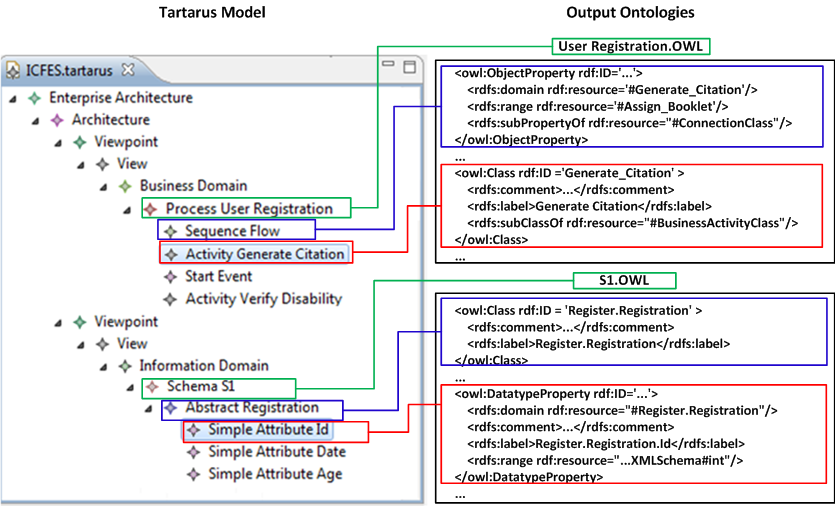
\includegraphics[scale=0.6,natwidth=835, natheight=506pt]{OWL_trans.png}
	\caption{Ejemplo de Transformaci\'on Tartarus-OWL}
	\label{fig:Transform}
\end{center}	
\end{figure*}
%........................................................
%===============================================================
\subsection{Matching de Ontolog\'ias} \label{sec:alignstep}
%===============================================================
En esta fase se infiere la trazabilidad y redundancia en los dominios BA-IA. Se procesan mediante un motor de matching las ontolog\'ias generadas en el paso anterior. Definimos dos tipos de tareas de matching de ontolog\'ias en el \'ambito de Kalcas: Entre ontolog\'ias de dominios diferentes y entre ontolog\'ias del mismo dominio. Estas dos tipolog\'ias est\'an en l\'inea con las funciones $traceability(C_{i},C_{j})$ y $redundancy(C_{i},C_{j})$ definidas en la Secci\'on \ref{sec:conceptualization}. La Figura \ref{fig:alignmenttask} muestra la ejecuci\'on de los dos tipos de tareas de alineamiento.

%........................................................
\begin{figure} [!t]
\begin{center}
	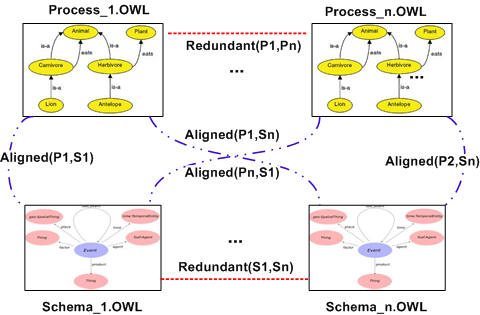
\includegraphics[scale=0.55,natwidth=480, natheight=315]{Schema_Alignment.png}
	\caption{Tipos de Tareas de Matching de Ontolog\'ias en Kalcas}
	\label{fig:alignmenttask}
\end{center}	
\end{figure}
%........................................................


La arquitectura de Kalcas utiliza el motor de alineamiento como un componente de software, por tanto es independiente a la implementaci\'on del motor de matching de ontolog\'ias. El motor de alineaci\'on utilizado en la versi\'on actual de Kalcas es \textit{Alignment API 4.3} disponible en \cite{AlignmentAPI:2012}. Esta API es una implementaci\'on para expresar, ejecutar y compartir alineamientos de ontolog\'ias \cite{David:2011}. Para cada pareja de ontolog\'ias, invocamos program\'aticamente \textit{Alignment API}, seleccionando un conjunto de comparadores que ya vienen implementadas dentro del API. Cada algoritmo debe ser configurado con par\'ametros como umbral de similitud. Estas t\'ecnicas, utilizan nombres, comentarios, etiquetas, tipos de dato y estructuras para determinar un grado de similitud (entre 0 y 1). Las correspondencias encontradas entre \textit{Abstract} y \textit{DataObject} son propagadas a las actividades asociadas a los \textit{DataObject} con el fin de trazar un puente entre actividades y entidades.

Todos los mapeos candidatos generados por el motor, son cargados de vuelta al modelo \textit{ICFES.tartarus} como elementos \textit{AttrMatch, ProcessMatch o BIAlignment} utilizando EMF en un estado pendiente (\textit{state=PENDING}) y con el \'indice de similitud calculado por el motor. Por ejemplo, la correspondencia inferida entre las entidades \textit{S1.Registration} y \textit{S2.Registered} es consignada en el modelo como el objeto \textit{AttrMatch : S1.Registration\_ S2.Registered} con atributos: \textit{left:S1.Registration, right:S2.Registered, sim:0.9, state:PENDING}. 

%........................................................
\begin{figure} [!t]
\begin{center}
	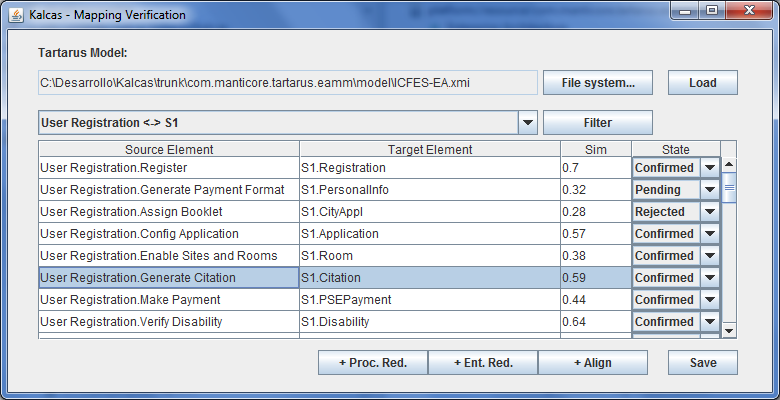
\includegraphics[scale=0.65,natwidth=783, natheight=399]{guiuser.png}
	\caption{GUI para Verificaci\'on de Mapeos Candidatos}
	\label{fig:Confirmation}
\end{center}	
\end{figure}
%........................................................

%===============================================================
\subsection{Verificaci\'on de Usuario}
%===============================================================

Una vez calculadas las alineaciones y redundancias candidatas, estas deben ser verificadas por el arquitecto.  Para tal fin, una interfaz gr\'afica de usuario (GUI) fue desarrollada con la librer\'ia Swing de Java y EMF para acceder y actualizar el modelo. Esta GUI permite seleccionar el modelo Tartarus, y una vez cargado se presenta una tabla con las correspondencias inferidas y su \'indice de similitud. El usuario puede confirmar o rechazar el mapeo como se ve en la Figura \ref{fig:Confirmation}. El prop\'osito de esta interfaz es ofrecer facilidades como filtros y ordenamientos para la gesti\'on de los mapeos candidatos. 

Tras la verificaci\'on del experto, los mapeos quedan en estado \textit{CONFIRMED} o \textit{REJECTED} dentro del modelo Tartarus. S\'olo los mapeos con confirmados son tenidos en cuenta en las consultas posteriores sobre el modelo.


%%===============================================================
\chapter{Realizando consultas con Kalcas Query Language}
 \label{cha:KQL}
%===============================================================

Como complemento a nuestra propuesta, definimos Kalcas Query Language (KQL), un DSL gr\'afico que permite realizar consultas sobre un modelo Tartarus utilizando la trazabilidad inferida y confirmada en el Cap\'itulo \ref{cha:solution}. KQL esta compuesto por dos metamodelos, uno para expresar consultas (KQLQuery) y otro que permite consignar la respuesta (KQLResponse). El modelo de consulta (conforme con KQLQuery) se entreteje con un modelo de EA (conforme con Tartarus) para obtener el modelo de respuesta (conforme con KQLResponse) aplicado a una EA particular. La respuesta al usuario se presenta como un grafo interpretado con la herramienta Graphviz, para lo cual se aplica una transformaci\'on del modelo KQLResponse a \texttt{dot}. La Figura \ref{fig:KQLTransform} describe como se transforman los diferentes modelos descritos para generar la respuesta a una consulta KQL. A continuaci\'on, vamos a describir con mayor detalle cada unos de los elementos involucrados.

%........................................................
\begin{figure} [!t]
\begin{center}
	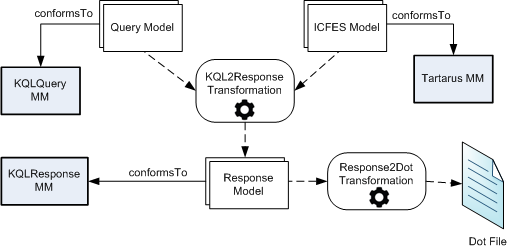
\includegraphics[scale=0.8,natwidth=507, natheight=248]{KQLTransform.png}
	\caption{Cadena de Transformaciones de Kalcas Query Language}
	\label{fig:KQLTransform}
\end{center}	
\end{figure}
%........................................................


%===============================================================
\section{Metamodelo KQLQuery}
%===============================================================

KQLQuery nos permite realizar consultas de alineaci\'on o redundancia sobre una determinada EA (modelo Tartarus), por ejemplo expresar las heur\'isticas introducidas en el Cap\'itulo \ref{cha:intro}. El metamodelo KQLQuery define los diferentes constructos del lenguaje que se pueden observar en la Figura \ref{fig:KQL_mm}. El elemento \texttt{Query} contiene las entradas de la consulta. Estas entradas pueden ser procesos y actividades en el dominio de negocio o esquemas y entidades en el dominio de informaci\'on. A partir de este metamodelo y utilizado la herramienta EuGENia \cite{Eugenia:2012} se genera un editor GMF (Graphical Modeling Framework) que permite expresar gr\'aficamente consultas en lenguaje KQLQuery. En la Figura \ref{fig:KQL_els} se puede ver el Editor KQL generado junto con los elementos que permiten dise\~nar las consultas.

%........................................................
\begin{figure} [!t]
\begin{center}
	\includegraphics[scale=0.47,natwidth=839, natheight=427pt]{KQL_mm.png}
	\caption{Metamodelo KQLQuery}
	\label{fig:KQL_mm}
\end{center}	
\end{figure}
%........................................................

%........................................................
\begin{figure} [!t]
\begin{center}
	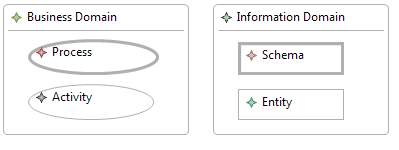
\includegraphics[scale=0.8, natwidth=399, natheight=150pt]{KQL_Elements.png}
	\caption{Elementos en el Editor KQL}
	\label{fig:KQL_els}
\end{center}	
\end{figure}
%........................................................

%........................................................
\begin{figure} [!t]
\begin{center}
	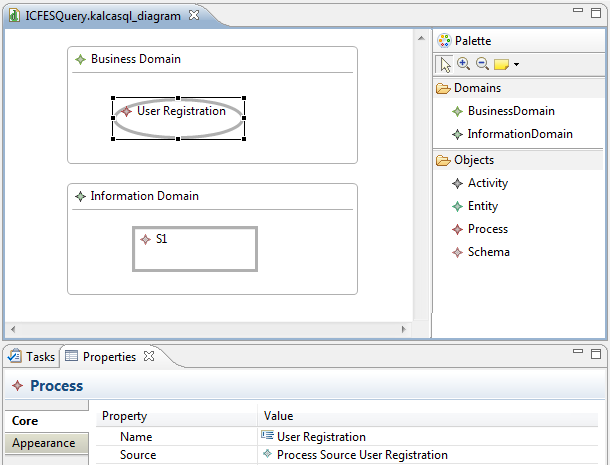
\includegraphics[scale=0.6,natwidth=610, natheight=465pt]{KQL_Question.png}
	\caption{Consulta de Alineamiento sobre el Editor KQL}
	\label{fig:KQL}
\end{center}	
\end{figure}
%........................................................


La gram\'atica KQLQuery comprende: Las secciones de dominio (Business - Information) ubicadas en la \textit{Zona de Trabajo} y los elementos de entrada en la \textit{Zona de Paleta}. Los elementos se arrastran desde la Paleta hasta las secciones de cada dominio para dise\~nar la consulta: \texttt{Process}, \texttt{Activity} (BA), \texttt{Schema} y \texttt{Entity} (IA). Estos componentes permiten definir la preguntas al modelo en t\'erminos de Negocio e Informaci\'on en diferente nivel de granularidad. Adem\'as, al definir la consulta, cada elemento puede tomar un valor no determinado \texttt{empty} (cualquier \texttt{Activity} o cualquier \texttt{Entity}) o un valor concreto del modelo (\texttt{Activity:Generar Citaci\'on} o \texttt{Entity:Citacion}). Unas vistas del editor generado se ofrecen en la Figuras \ref{fig:KQL} y \ref{fig:KQL_red}.

%........................................................
\begin{figure} [!t]
\begin{center}
	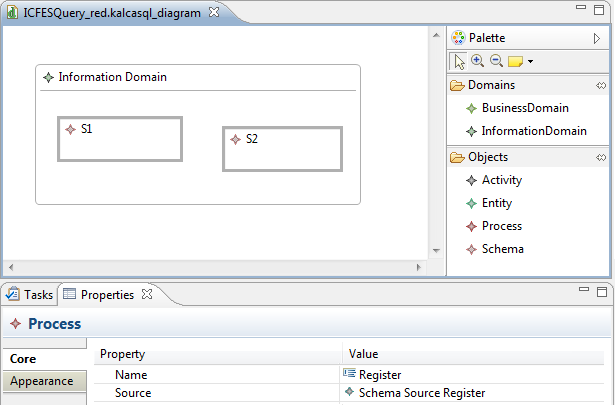
\includegraphics[scale=0.6,natwidth=612, natheight=405pt]{Redundancy_query.png}
	\caption{Consulta de Redundancia sobre el Editor KQL}
	\label{fig:KQL_red}
\end{center}	
\end{figure}
%........................................................

En la Figura \ref{fig:KQL} podemos observar una consulta de alineaci\'on (\texttt{ICFESQuery}) dise\~nada sobre nuestro caso de estudio. Se incluyen el proceso \texttt{User Registration} (Business Domain) y el Esquema \texttt{S1} (Information Domain) con el objetivo de conocer como est\'an alineados. Por otro lado, se puede ejecutar consultas de redundancias. Para este fin el usuario debe ubicar en la Secci\'on respectiva, los elementos de la paleta que desea analizar, por ejemplo en la Figura \ref{fig:KQL_red} se comparan los esquemas \texttt{Schema:S1} y \texttt{Schema:S2} en busca de redundancias. El editor gr\'afico al final construye un modelo KQLQuery que representa la pregunta que el arquitecto quiere hacer sobre el modelo Tartarus.

\section{Metamodelo KQLResponse}

El metamodelo KQLResponse presentado en la Figura \ref{fig:KQLResponse_mm} contiene los elementos resultantes de la intersecci\'on entre un modelo de consulta KQL y el modelo Tartarus. La consulta KQL se puede entender como una \textit{vista} sobre el modelo Tartatus que solo incluye los elementos involucrados y enriquecida con los conceptos de trazabilidad y redundancia. Al ser una vista parcial sobre Tartarus, el metamodelo KQLResponse tiene una estructura simplificada del metamodelo Tartarus. Encontramos las clases \texttt{InformationDomain} y \texttt{BusinessDomain}, los cuales contienen clases de tipo \texttt{Process} y/o \texttt{Schema}, mas las relaciones de redundancia (\texttt{AttrMatch} y \texttt{ProcessMatch}) o de trazabilidad (\texttt{BIAlignment}). 

Adicionalmente, como este metamodelo tiene tambi\'en prop\'ositos de an\'alisis gr\'afico, los conceptos \texttt{Entity} y \texttt{ProcessElement} poseen un atributo \texttt{aligntype} que determina, seg\'un la consulta, si el componente est\'a desalineado (\texttt{Misaligned}), alineado con un componente no incluido en la consulta (\texttt{OmittedAligned}), o alineado con un componente presente en la consulta (\texttt{Aligned}). Estas caracter\'isticas son representadas gr\'aficamente al usuario.

%........................................................
\begin{figure} [!t]
\begin{center}
	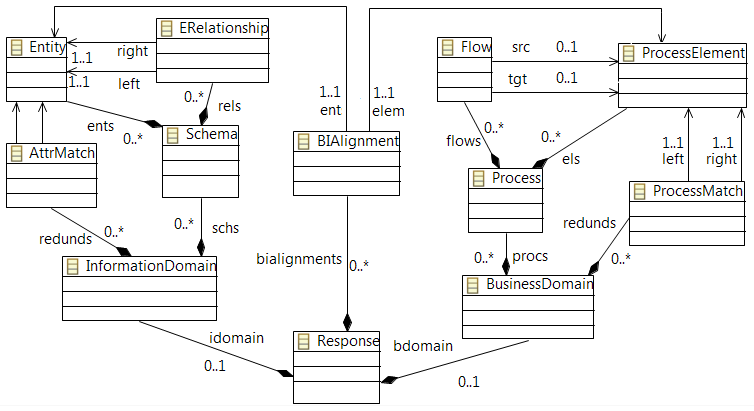
\includegraphics[scale=0.55,natwidth=754, natheight=411pt]{KQLResponse_mm.png}
	\caption{Metamodelo KQLResponse}
	\label{fig:KQLResponse_mm}
\end{center}	
\end{figure}
%........................................................

\section{Transformaci\'on Query2Response}

Para generar el modelo de respuesta conforme KQLResponse, se desarroll\'o una transformaci\'on ATL \cite{Jouault:2008} que toma de entrada los modelos KQLQuery y Tartarus para navegarlos y entretejerlos generando un modelo de salida. La transformaci\'on recorre los \texttt{Input} del modelo KQLQuery y va buscando los elementos asociados en el modelo Tartarus, con el fin de incluir todos los componentes relacionados con el elemento \texttt{Input}. 

Adicionalmente, a los objetos de clase \texttt{Activity} y \texttt{Entity} se les asigna el tipo de alineamiento (\texttt{aligntype}) de acuerdo a las alineaciones presentes en el modelo Tartarus y los criterios ingresados en el modelo de consulta. Continuando con nuestro caso de estudio, al procesar la consulta expresada en la Figura \ref{fig:KQL}, la transformaci\'on extrae todos los elementos asociados al \texttt{Proceso de Registro}, al esquema \texttt{Registro} y las relaciones \texttt{BIAlignment} contenidas dentro del modelo \texttt{ICFES.tartarus} para generar un modelo de respuesta \texttt{ResponseICFES}.

\section{Transformaci\'on Response2Dot}

Una vez obtenido el modelo de respuesta, una transformaci\'on modelo a texto es implementada con una plantilla Xpand la cual genera un archivo \textit{dot} que contiene una representaci\'on gr\'afica del modelo de respuesta. \textit{dot} permite dibujar grafos leyendo archivos de texto y produciendo archivos gr\'aficos \cite{Koutsofios:2002}. 

Los dominios de Negocio e Informaci\'on consignados en modelo KQLResponse se transforman a Cluster dentro del archivo dot. Similarmente los procesos y esquemas tambi\'en se convierten en subclusters contenidos dentro de los cluster principales (BusinessDomain o InformationDomain). Por otro lado, los ProcessElement ( i.e. \texttt{Activity, Gateway, Event}) y Entity se traducen en nodos con colores que representan su tipo de alineamiento (i.e. \texttt{Aligned=green, OmittedAligned=yellow, Misaligned=red}). Las relaciones inferidas (trazabilidad o redundancia) se representan con l\'ineas punteadas y las relaciones que ya vienen dadas desde los modelos importados (BPMN y ER) se dibujan con l\'ineas continuas. 

\begin{lstlisting}[caption={Segment of output dot file},label=lst:dot, basicstyle=\small, tabsize=2,morekeywords={digraph, subgraph, -> }]
digraph G{
subgraph cluster0 {
	label = "Business Domain";
subgraph cluster_User_Registration {
	label = "User Registration";
	Generate_Citation
	[label="Generate\nCitation", shape=box, 
	style="filled,rounded", color=green];
...
}
}
subgraph cluster1 {
	label = "Information Domain";
subgraph cluster_S1 {
		label = "S1";
		Citation [label="Citation", 
		shape=box, style="filled", color=green ];
...
}
}		
	Citation -> 
	User_Registration[style=dashed];
}	
\end{lstlisting}

\begin{landscape}
 
%........................................................
\begin{figure} 
\begin{center}
	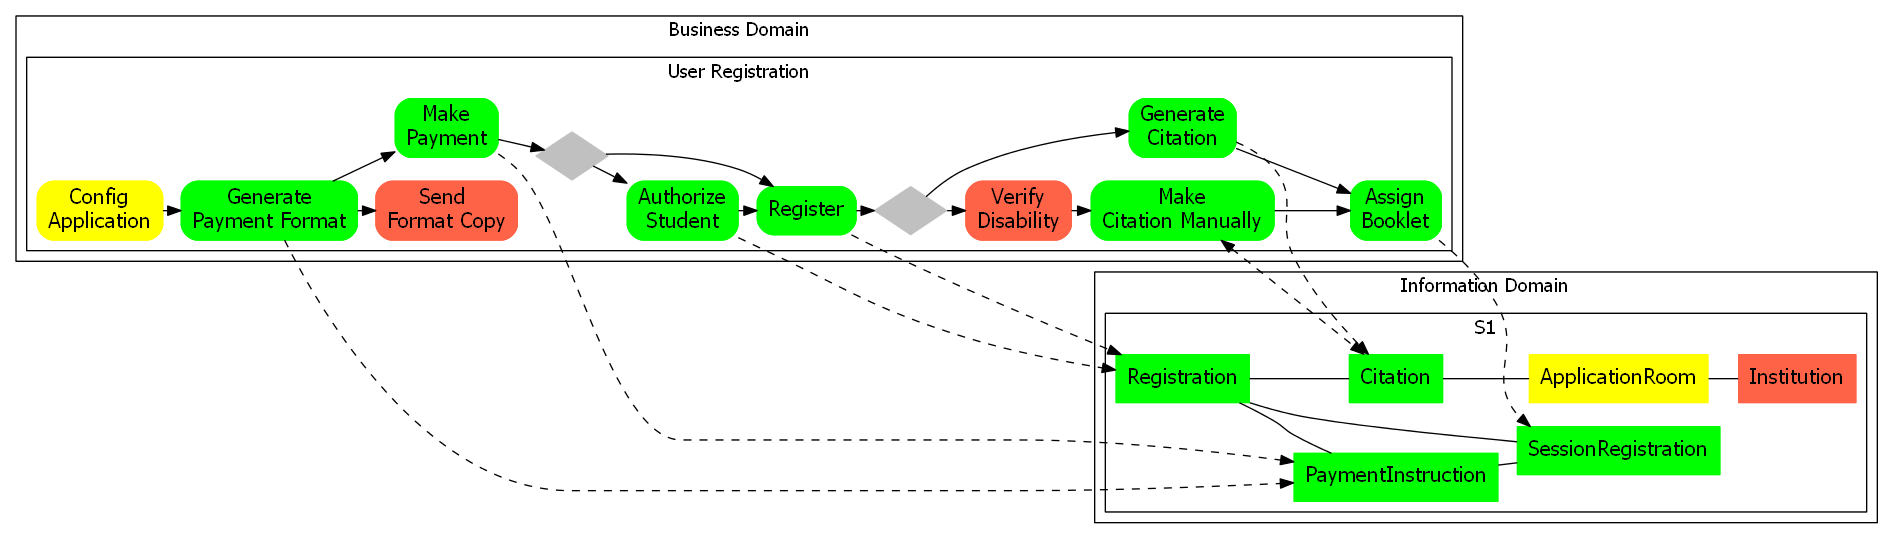
\includegraphics[scale=0.3,natwidth=1893, natheight=539pt]{align.png}
	\caption{Salida de una Consulta de Alineamiento en KQL}
	\label{fig:KQL_out}
\end{center}	
\end{figure}
%........................................................

%........................................................
\begin{figure} [!t]
\begin{center}
	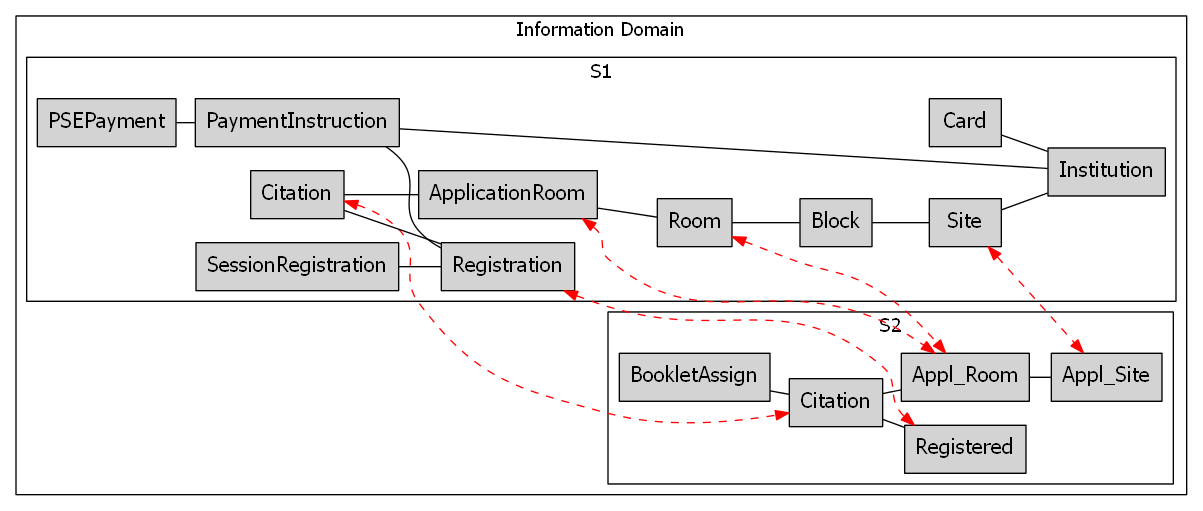
\includegraphics[scale=0.3,natwidth=1349, natheight=591pt]{redund.png}
	\caption{Salida de una Consulta de Redundancia en KQL}
	\label{fig:KQL_out2}
\end{center}	
\end{figure}
%........................................................

\end{landscape}

El Listado \ref{lst:dot} es un segmento del archivo dot de salida donde se puede apreciar la estructura jer\'arquica de clusters, as\'i como los componentes de cada dominio enriquecidos con elementos gr\'aficos. Este archivo dot es interpretado por Graphviz y genera la imagen que se presenta en la Figura \ref{fig:KQL_out}. La imagen corresponde a la consulta expresada en previamente en la Figura \ref{fig:KQL}. Este reporte permite identificar los procesos que no tienen trazabilidad en el dominio de informaci\'on y viceversa. Otro ejemplo es la salida de la consulta de redundancia dise\~nada en la Figura \ref{fig:KQL_red} que se presenta en la Figura \ref{fig:KQL_out2}.

Tanto los objetos que aparecen \texttt{Misaligned} al ejecutar una \texttt{Alignment Query} (i.e. actividad \texttt{Send Format Copy} y entidad \texttt{Institucion}) como los objetos incluidos en el resultado de una \textit{Redundancy Query} (i.e. Entidades Citation) constituyen los potenciales desalineamientos evaluados por las heur\'isticas referidas en el Cap\'itulo \ref{cha:intro}.
%%=================================================================
\chapter{IMPLEMENTACI\'ON DE LA PROPUESTA} \label{cha:implementacion}
%=================================================================

Kalcas fue desarrollado con el IDE Eclipse y construido sobre Eclipse Modelling Framework (EMF). Toda la implementaci\'on se divide en seis grupos de proyectos Eclipse que se muestran en la Figura \ref{fig:projects}. El primer proyecto contiene el metamodelo ecore de EA. El segundo proyecto \textit{tartarus.serializer} contiene los importadores tanto de procesos de negocio como de esquemas de base de datos. El tercero \textit{tartarus.transformation} contiene las plantillas Xpand que genera los archivos OWL a partir del modelo Tartarus. Los proyectos \textit{co.edu.uniandes.kalcasql} corresponden a los proyectos GMF que generan el editor gr\'afico KQL. El proyecto \textit{co.edu.uniandes.kalcas.tartarus2kalcas} genera el modelo de respuesta para una consulta hecha en KQL. Por \'ultimo, \textit{co.edu.uniandes.kalcas.kalcas2gv} contiene la transformaci\'on XPand que genera el archivo dot a partir de la respuesta generada. La Figura \ref{fig:arch} ofrece una vista general de la arquitectura de Kalcas. A continuaci\'on se explican con mayor detalle los proyectos en que se ha implementado nuestra aproximaci\'on.

%--------------------------------------------------------------------------------------
\begin{figure}[!t]
\begin{center}
	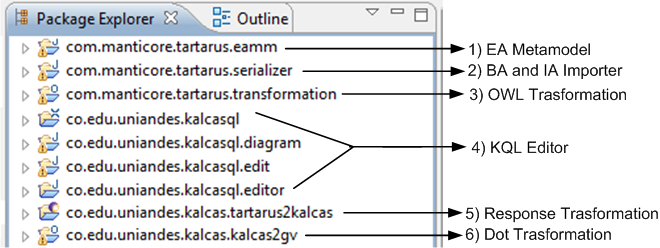
\includegraphics[scale=0.5 ,natwidth=660pt, natheight=248pt]{projects.png}
	\caption{Proyectos Eclipse}
	\label{fig:projects}
\end{center}
\end{figure} 
%--------------------------------------------------------------------------------------

%--------------------------------------------------------------------------------------
\begin{figure}[!t]
\begin{center}
	\includegraphics[scale=0.5 ,natwidth=684pt, natheight=281pt]{kalcas_arch.png}
	\caption{Arquitectura Kalcas}
	\label{fig:arch}
\end{center}
\end{figure} 
%--------------------------------------------------------------------------------------


\begin{enumerate}

\item El proyecto \textit{tartarus.eamm} contiene el metamodelo ecore de Tartarus y los modelos xmi conformes a Tartarus. Adicionalmente, en este proyecto tambi\'en est\'an las clases java que representan los conceptos del metamodelo y permiten leer y editar program\'aticamente los modelos conformes con Tartarus. Este proyecto tambi\'en incluye el paquete \textit{matching.align} el cual funciona como interfaz con el motor de alineamiento \textit{AlignmentAPI}. Sobre el archivo \textit{matching.properties} se configuran la ruta de las ontolog\'ias a procesar y el modelo Tartarus donde se registrar\'an los mapeos inferidos. Dentro de este proyecto tambi\'en se encuentra el paquete java \textit{kalcas.verification} que implementa una GUI utilizando la librer\'ia \textit{javax.swing}. Esta GUI permite a un usuario confirmar los mapeos inferidos.

\item Los importadores de BA e IA se localizan en el proyecto \textit{tartarus.serializer}. Clases Java utilizan el API Xstream para acceder los archivos XPDL que describen la BA y las procesan para convertirlas en conceptos Tartarus. Para tal fin, un archivo de propiedades (TartarusSerializer.properties) permite definir la ruta de los archivos fuentes y el modelo Tartarus de destino. En el caso de la IA, se accede program\'aticamente a los esquemas a trav\'es de un conector JDBC y la librer\'ia \textit{java.sql}. Los par\'ametros para conectarse a la base de datos son al igual configurados en archivos de propiedades. Estos importadores generan o actualizan el modelo XMI conforme con Tararus con la informaci\'on contenida en procesos y esquemas.

\item Dentro de \texttt{tartarus.transformation} est\'a la plantilla \textit{Process2RDFXML.xpt} en lenguaje Xpand que se encarga de recorrer el modelo Tartarus para generar ontolog\'ias OWL para cada proceso de la BA. Similarmente la plantilla \textit{Schema2RDFXML.xpt} transforma los esquemas y sus entidades en ontolog\'ias OWL.  Cada plantilla es ejecutada mediante un Motor de Workflow de Modelamiento(Modeling Workflow Engine (GenerateOWLFromProcess.mwe y GenerateOWLFromSchema.mwe). Las ontolog\'ias de salida son generadas en la carpeta src-gen/ para ser procesadas posteriormente.

\item Los proyectos \textit{kalcasql} son los que en conjunto implementan el editor KQL. El proyecto \textit{kalcasql} contiene el metamodelo \textit{kalcasql.ecore} y los modelos intermedios GMF. Los proyectos \textit{diagram, edit} y \textit{editor} comprenden las clases java que implementan el plugin KQLEditor y fueron generadas mediante EuGENia. El editor KQL se ejecuta como una instancia eclipse que el usuario utiliza para dise\~nar las consultas.

\item \textit{Tartarus2kalcas} es un proyecto \textit{ATL} que contiene la transformaci\'on \texttt{query2response.atl} la cual toma un modelo Tartarus y un modelo KQLQuery para procesarlos y generar un modelo de salida conforme con el metamodelo KQLResponse. Este modelo de respuesta es transformado a texto posteriormente.

\item El proyecto \textit{kalcas2gv} contiene el metamodelo KQLResponse.ecore y sus diferentes modelos que representan las respuestas generadas a consultas KQL. Adicionalmente, la plantilla \textit{kalcasql2dot.xpt} implementada en XPand se encarga de realizar la transformaci\'on del modelo de respuesta a un archivo dot. Los archivos dot son generados en la carpeta \textit{src-gen}. Cada archivo dot es interpretado por la herramienta Graphviz y presentado en formato gr\'afico.

\end{enumerate}
%%=================================================================
\chapter{Validaci\'on del Caso de Estudio} \label{cha:evaluation}
%=================================================================

%**************************************************************
\section{Introducci\'on} \label{sec:evalintro}
%**************************************************************

El desarrollo total de Kalcas tom\'o dos semestres acad\'emicos de trabajo con una dedicaci\'on de medio tiempo. Se invirtieron tres meses en la revisi\'on bibliogr\'afica sobre la evaluaci\'on de alineaci\'on en el marco de EA y modelos de dominio de EA. Posteriormente tomamos dos meses mas analizando la aplicaci\'on de ontolog\'ias y razonadores en el contexto de la evaluaci\'on de alineaci\'on. Una vez tuvimos claro el planteamiento del problema y un propuesta de soluci\'on inicial construimos las herramientas necesarias durante los cuatro meses siguientes. En cada fase de la fase de construcci\'on fuimos refinando esta propuesta tanto conceptual como t\'ecnicamente hasta tener un framework funcional que nos permiti\'o validar nuestras hip\'otesis sobre un segmento de una EA real.  

Nuestro trabajo ha sido aplicado y validado en el Instituto Colombiano para la Evaluaci\'on de la Educaci\'on (ICFES). Para evaluar esta propuesta, definimos un experimento que involucra un segmento de la EA del ICFES compuesto por los dos procesos de negocio y esquemas introducidos en el Cap\'itulo \ref{cha:studycase}, mas un nuevo proceso encargado de la actualizaci\'on de los datos de las instituciones de educaci\'on b\'asica que ser\'an evaluadas.

Los procesos analizados fueron: User Registration (\textit{P1}), Corporate User Registration (\textit{P2}) y Data Updating of Saber359 (\textit{P3}) los cuales hacen parte de la vertical de negocio. Dado que el ICFES es la \'unica organizaci\'on en Colombia autorizada por el gobierno para evaluar la calidad de la educaci\'on, las aplicaciones y esquemas que los soportan fueron construidos \textit{in house} y a la medida. Estos procesos son los que con mayor frecuencia requieren an\'alisis, ajustes y refinamientos debido a la transformaci\'on reciente del Instituto y el dinamismo propio del negocio. Estos tres procesos son soportados por tres esquemas de base de datos, a los cuales nos referiremos por su c\'odigo por razones de confidencialidad: \textit{S1}, \textit{S2} y \textit{S3}. La complejidad de los procesos est\'a dada por la cantidad de actividades que los componen. El proceso \texttt{P1} contiene 18 actividades, \texttt{P2} involucra 9 actividades y \texttt{P3} comprende 12 actividades. La complejidad de los esquemas subyacentes esta dada por la cantidad de entidades que contienen: \texttt{S1} tiene 27 tablas, \texttt{S2} tiene 8 tablas y \texttt{S3} 8 tablas.

La validaci\'on de nuestra propuesta est\'a basada en la medici\'on de exactitud al realizar tres tareas de an\'alisis por parte de los arquitectos sobre el segmento de la EA del ICFES. Las tres tareas de an\'alisis fueron: Definir la trazabilidad entre BA-IA (\texttt{T1}), identificar desalineaciones BA-IA (\texttt{T2}) e identificar redundancias de procesos en BA y de entidades en IA (\texttt{T3}). En este experimento tambi\'en comparamos los tiempos invertidos en los an\'alisis de cada tarea, aclarando que a priori asumimos que el proceso manual en general tarda mas que un proceso automatizado, por tanto nuestra intenci\'on se enfoc\'o en verificar en la pr\'actica los niveles de reducci\'on de tiempos para cada tarea y cada proceso.

Para explicar mejor la medida de exactitud dentro nuestro experimento es necesario introducir los conceptos \textit{precisi\'on, exhaustividad} y \textit{F-Measure}:

La precisi\'on (\textit{precision}) se refiere a la fidelidad y da cuenta de la proporci\'on de elementos efectivos sobre el total de elementos recuperados. La exhaustividad (\textit{recall}) est\'a asociada con la completitud y mide la raz\'on entre el total de elementos recuperados sobre el total de elementos que debieron ser identificados. Estos valores se calculan a la luz de un \textit{Alineamiento de Referencia}, el cual es un alineamiento hecho manualmente que se asume \textit{ideal} y que es realizado por un grupo de expertos. La exactitud de las tareas de an\'alisis en nuestra experimentaci\'on es cuantificada con la media arm\'onica \textit{F-Measure} que combina tanto \textit{precisi\'on} como \textit{exhaustividad} para determinar un balance entre estas variables y oscila entre \textit{0} y \textit{1}.

\begin{center}
	\begin{math}
	F-Measure = 2 \cdot{\frac{Precision\cdot{Recall}}{Precision+Recall}}
	\end{math}
\end{center}

Para esta experimentaci\'on nos apoyaron cuatro arquitectos del ICFES, quienes directamente trabajan en el proyecto de EA del instituto. Se les solicit\'o realizar las tareas \textit{T1, T2} y \textit{T3} con las herramientas que usan cotidianamente, y posteriormente utilizaron Kalcas sobre las mismas tareas de an\'alisis.

\section{Hip\'otesis} \label{sec:hypothesis}

Nuestro dise\~no experimental se basa en la formulaci\'on de dos hip\'otesis nulas (\textit{H$_{10}$} y \textit{H$_{20}$}) que esperamos rechazar y dos hip\'otesis alternativas (\textit{H$_{11}$} y \textit{H$_{21}$}) que asumimos ser\'an aceptadas tras los resultados de la experimentaci\'on. Las hip\'otesis fueron derivadas de las preguntas de investigaci\'on propuestas en la Secci\'on \ref{sec:problem}.

\textbf{H$_{10}$:} La exactitud (\textit{F-Measure}) al realizar una tarea de an\'alisis de alineaci\'on entre BA-IA es igual cuando es soportada por herramientas tradicionales que cuando es apoyada por Kalcas. Sea $FM_{ea}(T_{x}, P_{i},S_{j},RA_{ij})$ la funci\'on que calcula la exactitud promedio de los arquitectos al realizar la tarea de an\'alisis $T_{x}$ apoyada por herramientas tradicionales sobre el proceso de negocio $P_{i}$ y el esquema $S_{j}$ evaluada contra la alineaci\'on de referencia $RA_{ij}$. Sea $FM_{k}(T_{x}, P_{i},S_{j},RA_{ij})$ la exactitud promedio de los arquitectos al realizar la tarea de an\'alisis $T_{x}$ apoyada por Kalcas sobre el proceso de negocio $P_{i}$ y el esquema $S_{j}$ evaluada contra la alineaci\'on de referencia $RA_{ij}$.

\begin{center}
	\begin{math}
 \forall{x,i,j}(F-M_{ea}(T_{x}, P_{i},S_{j},RA_{ij}) = F-M_{k}(T_{x}, P_{i},S_{j},RA_{ij}))
	\end{math}
\end{center}


\textbf{H$_{11}$:} La exactitud (\textit{F-Measure}) al realizar una tarea de an\'alisis de alineaci\'on entre BA-IA es menor cuando es soportada por herramientas tradicionales que cuando es apoyada por Kalcas. Sea $FM_{ea}(T_{x}, P_{i},S_{j},RA_{ij})$ la funci\'on que calcula la exactitud promedio de los arquitectos al realizar la tarea de an\'alisis $T_{x}$ apoyada por herramientas tradicionales sobre el proceso de negocio $P_{i}$ y el esquema $S_{j}$ evaluada contra la alineaci\'on de referencia $RA_{ij}$. Sea $FM_{k}(T_{x}, P_{i},S_{j},RA_{ij})$ la exactitud promedio de los arquitectos al realizar la tarea de an\'alisis $T_{x}$ apoyada por Kalcas sobre el proceso de negocio $P_{i}$ y el esquema $S_{j}$ evaluada contra la alineaci\'on de referencia $RA_{ij}$.

\begin{center}
	\begin{math}
 \forall{x,i,j}(F-M_{ea}(T_{x}, P_{i},S_{j},RA_{ij}) < F-M_{k}(T_{x}, P_{i},S_{j},RA_{ij}))
	\end{math}
\end{center}

\textbf{H$_{20}$:} El tiempo (\textit{t}) al realizar una tarea de an\'alisis de alineaci\'on entre BA-IA es igual cuando se soporta por herramientas tradicionales que cuando se apoya en Kalcas. Sea $Ti_{ea}(T_{x}, P_{i},S_{j})$ la funci\'on que calcula el tiempo promedio de los arquitectos al realizar la tarea de an\'alisis $T_{x}$ apoyada por herramientas tradicionales sobre el proceso de negocio $P_{i}$ y el esquema $S_{j}$. Sea $Ti_{k}(T_{x}, P_{i},S_{j})$ la funci\'on que calcula el tiempo promedio de los arquitectos al realizar la tarea de an\'alisis $T_{x}$ apoyada por Kalcas sobre el proceso de negocio $P_{i}$ y el esquema $S_{j}$.

\begin{center}
	\begin{math}
 \forall{x,i,j}(Ti_{ea}(T_{x}, P_{i},S_{j}) = Ti_{k}(T_{x}, P_{i},S_{j}))
	\end{math}
\end{center}

\textbf{H$_{21}$:} El tiempo (\textit{t}) al realizar una tarea de an\'alisis de alineaci\'on entre BA-IA es mayor cuando se soporta por herramientas tradicionales que cuando se apoya en Kalcas. Sea $Ti_{ea}(T_{x}, P_{i},S_{j})$ la funci\'on que calcula el tiempo promedio de los arquitectos al realizar la tarea de an\'alisis $T_{x}$ apoyada por herramientas tradicionales sobre el proceso de negocio $P_{i}$ y el esquema $S_{j}$. Sea $Ti_{k}(T_{x}, P_{i},S_{j})$ la funci\'on que calcula el tiempo promedio de los arquitectos al realizar la tarea de an\'alisis $T_{x}$ apoyada por Kalcas sobre el proceso de negocio $P_{i}$ y el esquema $S_{j}$.

\begin{center}
	\begin{math}
 \forall{x,i,j}(Ti_{ea}(T_{x}, P_{i},S_{j}) > Ti_{k}(T_{x}, P_{i},S_{j}))
	\end{math}
\end{center}



\subsection{Variables Independientes}

Nuestro experimento es conducido por cuatro variables independientes las cuales son las entradas del proceso de experimentaci\'on y se asumen invariables durante el experimento: 
\begin{itemize}
\item El n\'umero de elementos o componentes en cada proceso.
\item El n\'umero de elementos en cada esquema.
\item El conjunto de alineaci\'on de referencia que determina las relaciones de trazabilidad y redundancia correcta provista por un experto.
\end{itemize}

\subsection{Variables Dependientes}
El experimento utiliza cuatro variables dependientes que son las m\'etricas que resultan de la experimentaci\'on, las cuales nos permirit\'an rechazar o aprobar las hip\'otesis: 
\begin{itemize}
\item El conjunto de relaciones de trazabilidad y redundancia inferidas por Kalcas.
\item El conjunto de relaciones de trazabilidad y redundancia definidas por el grupo de arquitectos.
\item $F-M_{ea}$: La exactitud promedio en t\'erminos de F-Measure de las tareas de an\'alisis (\texttt{T1, T2, T3}) realizadas por los arquitectos apoyados con herramientas tradicionales.
\item $F-M_{k}$: La exactitud promedio en t\'erminos de F-Measure de las tareas de an\'alisis (\texttt{T1, T2, T3}) realizadas por los arquitectos apoyados con Kalcas.
\item $Ti_{ea}$: El tiempo promedio invertido en las tareas de an\'alisis (\texttt{T1, T2, T3}) realizadas por los arquitectos apoyados con herramientas tradicionales.
\item $Ti_{k}$:El tiempo promedio invertido en las tareas de an\'alisis (\texttt{T1, T2, T3}) realizadas por los arquitectos apoyados con Kalcas.
\end{itemize}

%**************************************************************
\section{Experimentaci\'on} \label{sec:experimentacion}
%**************************************************************

Se dise\~n\'o un cuestionario en una hoja de c\'alculo en el que los arquitectos respondieron preguntas asociadas las tareas \texttt{T1, T2} y \texttt{T3} apoyados en dos conjuntos de herramientas: \textit{Fase 1}: Las que se vienen utilizando dentro del instituto que incluyen Diagramas BPMN, Modelo Entidad-Relaci\'on y diccionarios de datos. \textit{Fase 2}: Por otro lado Kalcas Query Language. 

El cuestionario incluy\'o el tiempo consumido en cada tarea y preguntas puntuales sobre el segmento de EA analizado como: T1) Defina las relaciones de trazabilidad entre Actividades y Entidades para el proceso \texttt{Px} y el esquema \texttt{Sx}. T2.1) Identifique las actividades en el proceso \texttt{Px} que no est\'an soportadas por ninguna entidad de \texttt{Sx}. T2.2) Identifique para cada entidad de \texttt{Sx} del listado, la(s) actividad(es) soportada(s) por dicha entidad en el proceso \texttt{Px}. T3.1) Identifique las actividades redundantes entre los procesos \texttt{Px} y \texttt{Py}. T3.2 Para cada entidad en \texttt{Sx}, identifique las posibles entidades redundantes en cada esquema (\texttt{Sy y Sz}).


\subsection{Fase 1: Usando herramientas tradicionales} \label{subsec:exp-fase1}

Para esta primera fase, se realiz\'o una presentaci\'on a los participantes del experimento, explicando de forma general el objetivo del experimento, y los detalles propios del diligenciamiento de los cuestionarios. Los arquitectos contaron con artefactos de apoyo como diagramas BPMN de los procesos P1, P2 y P3 en versi\'on HTML que la herramienta Bizagi permite exportar. Tambi\'en contaron con el modelo entidad-relaci\'on en versi\'on HTML para facilitar la navegaci\'on y el acceso al detalle de tablas y campos. Este documento HTML contiene el detalle de los tipos de datos, comentarios y tama\~no de cada objeto dentro del esquema con el fin de habilitar la correcta realizaci\'on de las tareas \textit{T1, T2} y \textit{T3}.

Fue interesante observar como la primera tarea que individualmente realizaron los participantes fue trazar las l\'ineas que asociaban entidades y actividades para facilitar la resoluci\'on del conjunto de preguntas aplicadas, similar a la tarea que Kalcas aborda de manera semiautom\'atica. Una vez hechas las trazas, iniciaron a responder cada uno de los puntos del cuestionario. Esta fase se extendi\'o durante tres d\'ias trabajando de manera parcial y los tiempos invertidos quedaron especificados en los cuestionarios por cada tarea de an\'alisis. Al final el entregable de esta fase del experimento fueron las hojas de c\'alculo con los resultados de sus an\'alisis.

\subsection{Fase 2: Usando Kalcas} \label{subsec:exp-fase2}

En una segunda fase, se hizo uso de Kalcas sobre las mismas tareas de la fase anterior. La m\'aquina sobre la cual se realiz\'o el experimento con Kalcas es un laptop con procesador de doble n\'ucleo, 2.2 GHz de 64 bits y RAM de 4GB. Para el diligenciamiento del cuestionario usando Kalcas, se realiz\'o una capacitaci\'on de una hora a los arquitectos en el manejo del framework. 

Inicialmente, se importaron los tres procesos de negocios (\textit{P1, P2} y \textit{P3} en formato XPDL en 3.094 ms. Los esquemas \textit{S1, S2} y \textit{S2} que soportan estos procesos fueron cargados tambi\'en al modelo Tartarus en 56.312 ms desde una base de datos Oracle 10g por medio del importador JDBC-EMF.

El siguiente paso fue la ejecuci\'on de las transformaciones Tartarus-OWL, donde se generaron: Tres ontolog\'ias de esquemas y tres ontolog\'ias con los procesos de negocio. El tiempo de ejecuci\'on de estas transformaciones fue de 2.786 ms. Las quince tareas de matching (nueve comparaciones de trazabilidad y seis de redundancia) se realizaron en 476.188 ms, invocando de forma program\'atica los algoritmos ya incorporados en el motor \texttt{Alignment API}.

Los algoritmos de matching aplicados fueron \texttt{StringDistAlignment} y \texttt{JWNLAlignment} los cuales vienen implementados en la herramienta \textit{Alignment API}. El primero halla la distancia entre strings aplicando la distancia Levenshtein. El segundo se apoya en el l\'exico WordNet \cite{Miller:1995} para hallar similitudes ling\"u\'isticas a partir de sin\'onimos e hiper\'onimos. 

Una vez cargados los mapeos candidatos obtenidos, fueron verificados en la interfaz y actualizados en el modelo de EA. Esta tarea de verificaci\'on tom\'o alrededor de 40 minutos y nos permiti\'o evaluar la exactitud del motor de alineamiento como tal, contra un alineamiento de referencia con el prop\'osito de medir la calidad de las inferencias. En promedio el F-Measure de los mapeos inferidos antes de la fase de verificaci\'on fue de 0,5534. Los mapeos errados o no identificados por el motor fueron refinados en la etapa de confirmaci\'on por un experto.

Sobre el editor KQL realizaron consultas de alineamiento de prueba (\texttt{P1-S1}, \texttt{P2-S2} y \texttt{P1-S3}), el reporte de salida de la consulta \texttt{P1-S1} corresponde al grafo mostrado en la Figura \ref{fig:KQL_out}. Adicionalmente, ejecutamos consultas de redundancia (\texttt{P1-P2} y \texttt{S1-S2}) y la salida se puede observar en la Figura \ref{fig:KQL_out2}.

Posteriormente cada arquitecto complet\'o de nuevo todas las preguntas del cuestionario apoyado en las salidas que Kalcas presentaba a sus consultas. Tambi\'en se brind\'o soporte a los arquitectos sobre dudas puntuales en el uso del editor. Durante tres d\'ias a dedicaci\'on parcial, el grupo de arquitectos diligenci\'o el formulario con los resultados de sus inferencias. Para evitar sesgar los an\'alisis de cada arquitecto manejamos dos tipos de cuestionario que abordaban preguntas diferentes. De tal manera que el mismo arquitecto no respondiera exactamente las mismas preguntas en cada Fase. Aunque la BA e IA evaluadas eran las mismas, variamos las preguntas puntuales sobre determinadas entidades y actividades. Como en la fase anterior, las hojas de c\'alculo con los resultados de los an\'alisis y los tiempos invertidos fueron los resultados de esta fase.

\section{Resultados} \label{sec:evalresults}
%**************************************************************

Tabulamos los cuestionarios aplicados en las dos fases de experimentaci\'on y comparamos tiempos y exactitud de los an\'alisis con el indicador F-Measure abordado en la Secci\'on \ref{sec:evalintro}. 

La Figuras \ref{fig:time}, \ref{fig:time2} y \ref{fig:time3} presentan los tiempos promedio de cada tarea de alineamiento para cada proceso analizado. Se puede notar como disminuy\'o entre un 16\% y un 65\% el tiempo promedio invertido en realizar las tareas de an\'alisis. La mejora mas importante se puede evidenciar en la tarea \texttt{T1} realizada sobre el proceso mas complejo (\texttt{P1}), donde alcanzamos reducir de 28,5 a 10 minutos (65\%). Es importante anotar que en estas gr\'aficas no se est\'a incluyendo el tiempo de importaci\'on, matching de ontolog\'ias y confirmaci\'on de los mapeos que en total fue de 49 minutos para los tres procesos. La capacitaci\'on recibida por los arquitectos fue de dos horas en el manejo del editor KQL. 

Si tomamos la duraci\'on de las etapas investigaci\'on y desarrollo de Kalcas mencionados en la Secci\'on \ref{sec:evalintro}, sumado a los tiempos de capacitaci\'on de los arquitectos, encontramos que para el tama\~no de este experimento no resultar\'ia rentable en tiempo la aplicaci\'on de esta propuesta. Pero la ganancia est\'a en que la gran inversi\'on de recursos se realiza solo al inicio y por tanto los beneficios en t\'erminos de tiempo se obtienen en la utilizaci\'on de la herramienta en an\'alisis posteriores.


%........................................................
\begin{figure}[!t]
\begin{center}
	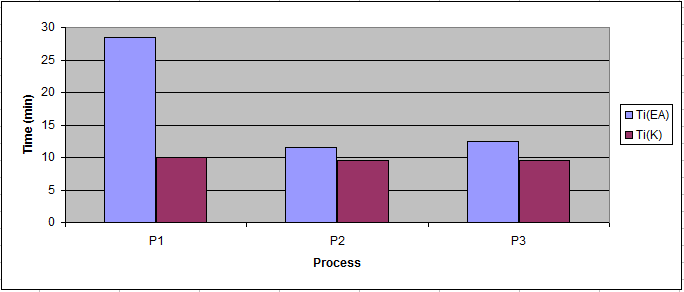
\includegraphics[scale=0.6 ,natwidth=682pt, natheight=290pt]{time.png}
	\caption{Promedios de Tiempo en la Tarea de An\'alisis 1}
	\label{fig:time}
\end{center}
\end{figure}

\begin{figure}[!t]
\begin{center}
	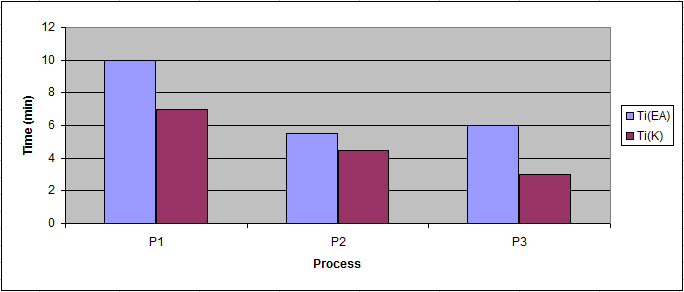
\includegraphics[scale=0.6 ,natwidth=682pt, natheight=291pt]{time2.png}
	\caption{Promedios de Tiempo en la Tarea de An\'alisis 2}
	\label{fig:time2}
\end{center}
\end{figure}

\begin{figure}[!t]
\begin{center}
	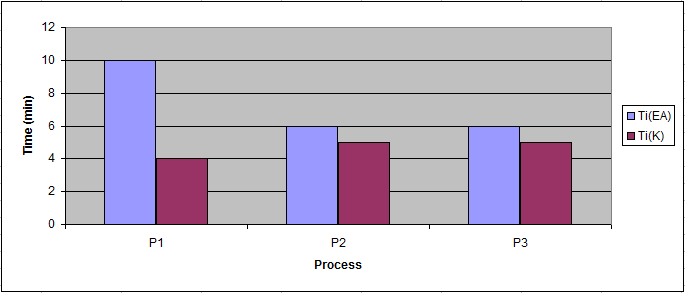
\includegraphics[scale=0.6 ,natwidth=684pt, natheight=292pt]{time3.png}
	\caption{Promedios de Tiempo en la Tarea de An\'alisis 3}
	\label{fig:time3}
\end{center}
\end{figure}

%........................................................

En la Figuras \ref{fig:results}, \ref{fig:results2} y \ref{fig:results3} se presenta el promedio de exactitud de todos los arquitectos realizando cada tareas sobre cada proceso. En cada Figura se compara para cada tarea (\texttt{T1, T2} y \texttt{T3}) la exactitud utilizando las herramientas tradicionales (\textit{EA}) y utilizando Kalcas \textit{K}.

%........................................................

\begin{figure}[!t]
\begin{center}
	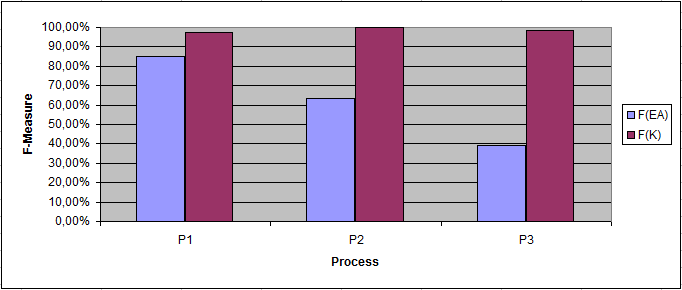
\includegraphics[scale=0.6 ,natwidth=682pt, natheight=289pt]{results.png}
	\caption{Promedios de Exactitud en la Tarea de An\'alisis 1}
	\label{fig:results}
\end{center}
\end{figure}

\begin{figure}[!t]
\begin{center}
	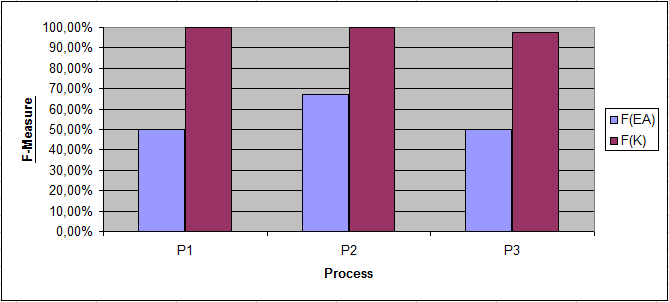
\includegraphics[scale=0.6 ,natwidth=669pt, natheight=302pt]{results2.png}
	\caption{Promedios de Exactitud en la Tarea de An\'alisis 2}
	\label{fig:results2}
\end{center}
\end{figure}

\begin{figure}[!t]
\begin{center}
	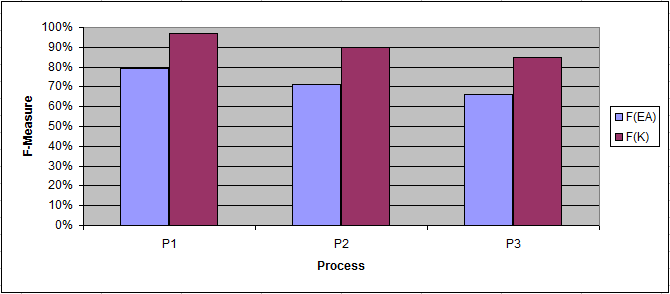
\includegraphics[scale=0.6 ,natwidth=669pt, natheight=293pt]{results3.png}
	\caption{Promedios de Exactitud en la Tarea de An\'alisis 3}
	\label{fig:results3}
\end{center}
\end{figure}

%........................................................

En general obtuvimos un aumento en la exactitud y por tanto una disminuci\'on de errores en las tareas de an\'alisis apoyadas en Kalcas. Particularmente, los mejores resultados en la tarea \texttt{T1} se obtuvo entre \texttt{P2-S2} y \texttt{P3-S3}, donde logramos aumentar la exactitud hasta en un 36\% y 59\% respectivamente. Tras analizar esta situaci\'on junto con los arquitectos, concluimos que la posible raz\'on es que el detalle del proceso \texttt{P1} es el m\'as conocido y socializado entre el grupo de arquitectos participantes, por tanto desde primera tarea de an\'alisis sin utilizar Kalcas ya se alcanz\'o un buen nivel de precisi\'on. Y por tanto Kalcas solo logr\'o refinarlo en un 11.9\%. Por otro lado, el detalle de los procesos \texttt{P2} y \texttt{P3} son menos conocidos por los arquitectos y de all\'i que Kalcas permiti\'o incrementar la exactitud en un 59\%. De manera similar la tarea \texttt{T2} al ser realizada utilizando Kalcas, present\'o mejoras entre el 32\% y el 50\% de exactitud. En cuanto a la tarea \texttt{T3} aunque tambi\'en present\'o mejoras fue la que evidenci\'o menores niveles de optimizaci\'on en el uso de Kalcas. Se alcanzaron incrementos entre un 17\% y 18.9\% de exactitud, siendo los procesos \texttt{P2} y \texttt{P3} los mas favorecidos (18.9\%).

Con los resultados obtenidos y volviendo sobre las hip\'otesis definidas en la Secci\'on \ref{sec:hypothesis} podemos concluir que la hip\'otesis H$_{11}$ es aceptada en cuanto el valor F-Measure fue menor para todos los casos soportados con Kalcas: H$_{10}$ - Rejected; H$_{11}$ - Accepted. La hip\'otesis H$_{21}$ es aceptada en cuanto el tiempo al realizar las tareas de an\'alisis fue menor cuando se apoyaron en Kalcas: H$_{20}$ - Rejected; H$_{21}$ - Accepted.

Con las tareas \texttt{T2} y \texttt{T3} pudimos expresar y evaluar las heur\'isticas descritas en el Cap\'itulo \ref{cha:intro}. Los resultados de evaluar los procesos y esquemas del ICFES con estas heur\'isticas se presentan en la Tabla \ref{tab:alignmentAB}.

\begin{table}
\begin{center}
\scalebox{1}{
\begin{tabular}{c c c} \hline
Heur\'istica Evaluada & Conjuntos Comparados & Hallazgos\\
\hline
Actividades que no acceden a ninguna entidad & P1-S1 & - \\
Actividades que no acceden a ninguna entidad & P2-S2 & 6 \\
Actividades que no acceden a ninguna entidad & P3-S3 & 6 \\
Entidades no accedidas por ninguna actividad & P1-S1 & 2 \\
Entidades no accedidas por ninguna actividad & P2-S2 & 1 \\
Entidades no accedidas por ninguna actividad & P3-S3 & 1 \\
Entidades redundantes & S1-S2 & 11	\\
Entidades redundantes & S1-S3 & 6 \\
Entidades redundantes & S2-S3 & 6 \\
Actividades redundantes & P1-P2 & 8 \\
Actividades redundantes & P1-P3 & 3 \\
Actividades redundantes & P2-P3 & 5 \\
\hline
\end{tabular}
}
\end{center}
\caption{Resultados de Evaluar Heur\'isticas de Desalineaci\'on}
\label{tab:alignmentAB}
\end{table}

Luego del an\'alisis de estos resultados, encontramos que los componentes redundantes detectados corresponden a procesos o entidades solapadas, dado que los dos procesos analizados son an\'alogos o por lo menos conceptualmente similares y por tanto tienen actividades y entidades en com\'un. La redundancia tanto de procesos como de entidades no implica un problema como tal, dado que bajo algunos escenarios la redundancia es conocida y hasta justificada, pero es importante identificar y evaluar dichos solapamientos. Los casos de objetos desalineados fueron analizados con mayor profundidad y llegamos a algunas conclusiones que ser\'an presentadas mas adelante en el Cap\'itulo \ref{cha:conclusions}.

Tras esta experimentaci\'on realizamos entrevistas con los arquitectos para recoger impresiones y aportes con respecto al uso de Kalcas, esto con el fin de retroalimentar esta propuesta desde un punto de vista mas cercano a la industria. Como ventajas, los usuarios resaltaron la agilidad y precisi\'on con la que Kalcas apoyaba sus an\'alsis sobre BA e IA. Tambi\'en fueron destacadas las opciones del editor para manejar a diferentes niveles de granularidad dentro de cada dominio, dado que se pod\'ian analizar procesos o esquemas completos o centrarse en entidades y actividades particulares. Como puntos a mejorar se recalc\'o la poca fluidez en los pasos para desplegar las herramientas y ejecutar las consultas. Esto debido a que las opciones para importar las arquitecturas, desplegar el editor KQL y ejecutar las consultas requer\'ian la configuraci\'on de archivos de propiedades, ejecuci\'on de instancias de eclipse y algunos pasos adicionales dentro del IDE para obtener los reportes de salida. Tenemos claro que la actual implementaci\'on requiere mas trabajo de integraci\'on y desarrollo de GUI para lograr ser utilizada adecuadamente en un entorno industrial. Otra posibilidad de mejora consiste en la legibilidad del reporte cuando se entra a analizar procesos o esquemas con gran cantidad de elementos, debido a que los diagramas de grafos generados en formato PNG por el algoritmo de Graphviz se tornan mas complejos y dif\'iciles de entender. En este punto se presentaron sugerencias como la exploraci\'on de reportes din\'amicos, que permitan navegar sobre el grafo, seleccionar y resaltar trazas de manera que se facilite la identificaci\'on de relaciones entre los conceptos. Para afrontar el problema de la complejidad, los arquitectos utilizaron la opci\'on de focalizar las consultas sobre determinadas entidades o actividades que eran objeto de an\'alisis. 

Finalmente, para el momento del experimento se hab\'ia llevando a cabo dentro del Instituto un proceso de mapear los procesos de negocio con las entidades, el cual fue costoso de realizar dado que tales relaciones no estaban formalizadas, sino en la mente de los arquitectos y analistas que participan en dichos procesos, y es all\'i donde la organizaci\'on vi\'o una oportunidad para obtener importantes aportes en la ejecuci\'on de tales tareas de alineamiento. Sumado a esto, la identificaci\'on de redundancias y desalineaciones sobre BA e IA le brind\'o un valor agregado al Instituto. En algunos casos para evidenciar algunos solapamientos que aunque no eran desconocidos, tampoco estaban formalmente identificados. En otros casos el experimento logr\'o identificar oportunidades en cuanto a mejorar la alineaci\'on en algunos componentes puntuales de la EA.
%%=================================================================
\chapter{TRABAJO RELACIONADO} \label{cha:relatedwork}
%=================================================================

Cuenca et al. \cite{Cuenca:2010} proponen un completo marco de modelamiento para la alineaci\'on Negocio-IT, que incluye las fases del ciclo de vida, modelo de madurez, vistas y artefactos. Su implementaci\'on se realiza a trav\'es de entrevistas y encuestas a expertos. En \cite{Plazaola:2008} se direcciona la evaluaci\'on de alineaci\'on Negocio-IT sobre EA como entrada para mejorar la toma de decisiones de alineamiento. Un metamodelo permite expresar criterios de calidad y evaluarlos utilizando reglas de inferencia para cuantificar un nivel de madurez de la organizaci\'on. La recolecci\'on de los datos del modelo de entrada se hace a mediante encuestas. Elhari y Bounabat \cite{Elhari:2011} presentan una plataforma para evaluar la alineaci\'on usando EA basada en un conjunto de m\'etricas que determinan un nivel de madurez de alineaci\'on. Este trabajo se soporta en la aplicaci\'on de encuestas para calcular dichas m\'etricas. Los datos de entrada de los modelos anteriores se resumen en encuestas y entrevistas a expertos. Nuestra propuesta, en cambio, toma como datos de entrada las definiciones formales de la EA para inferir trazas y medir la alineaci\'on, de tal manera que esperamos obtener resultados m\'as puntuales y objetivos. Kalcas actualmente tiene un alcance mas reducido dado que se focaliza solo en BA e IA y no en todos los dominios de la EA, pero Kalcas aporta mayor automatizaci\'on al inferir trazabilidad. 

En \cite{Aversano:2005} se propone a estrategia para ser aplicada durante la evoluci\'on para detectar desalineamientos entre procesos de negocio y los IS que los soportan. La estrategia es identificar los objetos que deben ser modificados para restaurar el alineamiento y considera un conjunto de atributos que representan indicadores de posible desalineamiento basados en an\'alisis de impacto. Una grafo de dependencia entre procesos de negocio e IS debe existir previamente para posibilitar el an\'alisis de impacto. Este grafo de dependencia es an\'alogo a la trazabilidad que buscamos inferir con nuestra aproximaci\'on. Kalcas no propone ajustes para restaurar el alineamiento solo evidencia los posibles desalineamientos entre BA-IA de una manera automatizada. En nuestro caso, el grafo de dependencia no est\'a dado, sino es inferido a trav\'es del matching de ontolog\'ias.

En \cite{Wegmann:2005} se introduce el marco te\'orico SEAM (Systemic Enterprise Architecture) y una herramienta asociada (SeamCAD) que chequea la alineaci\'on a trav\'es de la comparaci\'on de modelos descritos en t\'erminos de jerarqu\'ias funcionales y organizacionales. Esta propuesta requiere la definici\'on expl\'icita de las relaciones entre los diferentes componentes. La terminolog\'ia de SEAM est\'a basada en \textit{Reference Model for Open Distributed Processing} (RM-ODP) e implementada en una ontolog\'ia que permite usar m\'etodos formales de razonamiento. SEAM es aplicado en tiempo de dise\~no de la arquitectura para promover el alineamiento. La propuesta de Wegmann al igual que Kalcas utiliza razonamientos basados en ontolog\'ias de dominio espec\'ifico. Pero Kalcas est\'a enfocado en an\'alisis sobre BA e IA ya construidas, no pretende ser un nuevo lenguaje con el cual modelar arquitecturas de datos y procesos. Adicionalmente, Kalcas puede ser aplicado tanto en tiempo de dise\~no como de ejecuci\'on, dado que puede utilizarse sobre la arquitectura actual u objetivo.

Un framework propuesto por el grupo CEO (\textit{Centro de Engenharia Organizacional}) se describe en \cite{Vasconcelos:2007} como un conjunto de primitivas de modelamiento para expresar EA, Arquitectura de IS, Arquitectura de Software y las dependencias entre entre ellas. Adem\'as se definen un conjunto de m\'etricas que se eval\'uan autom\'aticamente para darle al arquitecto un conjunto de indicadores sobre el impacto de cada una de sus decisiones durante el proceso de construir una Arquitectura de IS. El Framework CEO apunta a proveer una descripci\'on formal de objetivos de negocio, procesos, recursos y SI. El lenguaje de modelamiento usado para implementar CEO fue UML, por lo cual se extendi\'o a trav\'es de estereotipos para hacer mas clara la identificaci\'on de los conceptos de negocio. Kalcas est\'a soportado en un metamodelo de EA, por tanto tambi\'en hace uso de un lenguaje para la expresi\'on de conceptos del dominio de la EA. Desde ese punto de vista, CEO tiene la ventaja de ser compatible con UML requerir\'ia transformaciones adicionales para hacerlo compatible con UML y poder ser utilizado por herramientas que soportan dicho lenguaje. A pesar que Kalcas tiene la informaci\'on necesaria para calcular m\'etricas, de momento no genera indicadores de alineaci\'on. De otro lado, Kalcas mas que un modelador, utiliza ingenier\'ia inversa sobre modelos ya existentes e infiere las relaciones entre tales modelos.

El trabajo de \cite{Simonin:2007} est\'a enmarcado en el desarrollo iterativo de servicios en \textit{France-Telecom}, el cual est\'a basado en \textit{Unified Process} (UP). La propuesta se apoya en MDA para medir en cada iteraci\'on de dise\~no de servicio el alineamiento entre requerimientos funcionales y la IA. Cuando se dise\~nan los servicios, los requerimientos funcionales son asociados a las entidades de negocio por el arquitecto. M\'etricas de alineamiento son propuestas para evaluar la perdida de informaci\'on entre el an\'alisis de requerimientos funcionales y el dise\~no de la IA. Estas m\'etricas son usadas en el contexto de un proceso de dise\~no iterativo para ayudar al arquitecto a seleccionar la mejor soluci\'on entre dos iteraciones. En com\'un, ambas propuestas involucra el modelo de la IA, pero Kalcas no aborda el an\'alisis de requerimientos sino los procesos de negocio de la compa\~nia. Nuestro trabajo asume que el dise\~no de la EA no incluy\'o un mecanismo de trazabilidad inicialmente, sino pretende inferir la trazabilidad en una EA ya construida. El uso de MDA para formalizar las definiciones est\'a presente tanto en \cite{Simonin:2007} como en Kalcas, pero el primero se apoya en reglas de transfomaci\'on de modelos para hallar inconsistencias, mientras que nuestro trabajo utiliza el razonamiento basado en ontolog\'ias. 

ArchiMate \cite{Jonkers:2004} es uno de los lenguajes de modelamiento de integraci\'on de EA mas difundidos y permite expresar a trav\'es de notaciones las relaciones que se dan entre los componentes de diferentes dominios de la EA. Nuestra aproximaci\'on no asume como preexistente la trazabilidad entre los dominios arquitecturales, sino pretende inferirlas a partir de las definiciones contenidas en la EA. Archimate aborda trazabilidad entre todos los dominios de la EA, Kalcas en su versi\'on actual solo incluye elementos de BA e IA. Y como en los casos anteriores, nuestro objetivo es ofrecer una herramienta para la evaluaci\'on del un modelo existente y no un lenguaje de modelamiento como tal.

En \cite{Pereira:2003, Pereira:2005, Sousa:2005} se eval\'ua la alineaci\'on mediante la verificaci\'on de heur\'isticas propuestas que deben cumplirse entre los diferentes dominios de la EA. Por ejemplo entre procesos y dato: Todos los procesos crean, actualizan y/o borran al menos una entidad; Todas las entidades son le\'idas al menos por un proceso; Entre procesos y aplicaciones: Cada proceso de negocio deber\'ia ser soportado por al menos una aplicaci\'on; Las tareas de los procesos de negocio deber\'ian ser soportadas por una sola aplicaci\'on; Procesos de negocio cr\'iticos deber\'ian depender de aplicaciones escalables y con alta disponibilidad. Aunque el trabajo propone heur\'isticas entre los dominios de IA, BA, AA y TA, no aborda una herramienta para realizar verificaciones de estas heur\'isticas, luego asumen revisiones manuales. Nuestra definici\'on de desalineaci\'on se basa en las heur\'isticas presentadas en estos trabajos, limit\'andose a evaluar solo a BA e IA. Nuestro trabajo habilita la expresi\'on y evaluaci\'on de estas heur\'isticas mediante KQL apoyando as\'i las tareas del arquitecto.

Otros trabajos han propuesto diferentes mecanismos para comparar componentes de la BA. En \cite{Remco:2009} se propone la aplicaci\'on de alineaciones basadas en grafos y l\'exicos para encontrar actividades similares en modelos de procesos de negocio. Por otro lado, una propuesta para expresar procesos de negocios con redes de Petri sobre ontolog\'ias se expone en \cite{Brockmans:2006} y su objetivo es realizar alineaciones sem\'anticas para soportar interconectividad semiautom\'atica de procesos de negocio. Por otro lado en \cite{Rodriguez:2011} se hallan diferencias entre dos versiones de un mismo proceso de negocio calculando el delta entre modelos. La coincidencia de estos trabajos con Kalcas, radica en que todos permiten detectar similitudes entre procesos de negocio utilizando modelos enriquecidos. Adicionalmente, con Kalcas exploramos el uso de matching de ontolog\'ias para hallar coincidencias entre activos de informaci\'on y relaciones de trazabilidad entre entre BA e IA. Junto con el trabajo de Rodr\'iguez \cite{Rodriguez:2011} compartimos el metamodelo Tartarus como n\'ucleo de nuestra propuesta, pero nuestros razonamientos utilizan ontolog\'ias a cambio de encontrar diferencias entre modelos.

La investigaci\'on documentada en \cite{Murcia:2011} tambien se apoy\'o en el metamodelo Tartarus para inferir redundancias dentro de una IA. Al igual que nuestra propuesta, se soport\'o en matching de ontolog\'ias para hallar tales redundancias, en particular el motor de alineamiento utilizado fue AgreementMaker \cite{Cruz:2009}. El trabajo all\'i presentado fue una fase previa a Kalcas y tienen en com\'un el uso de ontolog\'ias para inferir relaciones. Una vez hechas las inferencias, estas se presentan a manera de tablas HTML indicando el porcentaje de similitud. Dado que Kalcas es una continuaci\'on del trabajo propuesto por Murcia, nosotros reutilizamos algunos elementos como el importador de IA y la transformaci\'on de IA a ontolog\'ias. Comparado con Kalcas, el trabajo se limita a la detecci\'on de redundancias en IA, no aborda el concepto de alineamiento y carece de una herramienta para dise\~nar y ejecutar consultas sobre los modelos Tartarus.

El trabajo de tesis publicado en \cite{Moya:2012} aborda el alineamiento de Negocio e IT enfocado en la definici\'on de relaciones entre los pilares de Ross \cite{Ross:2006} y los conceptos presentados por Henderson y Venkatraman \cite{henderson:1990}. Una aproximaci\'on MDA de los pilares: Modelo Operacional, EA e Infraestructura de IT permite la definici\'on de alineamiento como el conjunto de relaciones que existe entre tales pilares. Al igual que Kalcas, el trabajo incluye la definici\'on de un DSL gr\'afico que soporta el dise\~no y ejecuci\'on de consultas de alineamiento sobre el metamodelo \textit{Tarmivol}. \textit{Tarmivol} permite integrar los metamodelos \textit{Tartarus}, \textit{Millo} (Metamodelo de procesos de negocio) y \textit{Archivol} (Metamodelo de arquitecturas de soluci\'on). La propuesta de Tarmivol tiene un espectro mas amplio comparada con Kalcas, dado que incluye los dem\'as dominios de la EA. Pero por otro lado es menos efectiva al inferir las relaciones de trazabilidad y alineaci\'on  porque solo tiene en cuenta elementos que sean textualmente exactos. Kalcas en cambio, se apoya en razonadores que logran inferencias mas complejas entendiendo que en el mundo real los componentes de BA e IA dif\'icilmente poseen nombres exactamente iguales.

%%=================================================================
\chapter{DISCUSI\'ON} \label{cha:conclusions}
%=================================================================

En este cap\'itulo discutimos los resultados, las conclusiones y limitaciones de este trabajo. Igualmente resumimos como esta propuesta aborda la problem\'atica presentada inicialmente y enumeramos las publicaciones realizadas en el desarrollo de este trabajo.

Inicialmente describimos el contexto de alineaci\'on entre Negocio y TI, algunas de las aproximaciones existentes y sus correspondientes problem\'aticas. Luego, presentamos una propuesta para apoyar la evaluaci\'on de alineaci\'on entre BA e IA utilizando MDA y matching de ontolog\'ias. Implementamos un conjunto de herramientas que ofrecen ingenier\'ia inversa de BA e IA, inferencia de trazabilidad y dise\~no de consultas. La tarea de matching autom\'atico de ontolog\'ias ofreci\'o un 55\% de exactitud, una invetigaci\'on mas profunda acerca de las t\'ecnicas y algoritmos utilizados puede aportar mayor precisi\'on en esta fase.

Formalizamos la trazabilidad, redundancia y alineamiento con el prop\'osito de dar las bases para construir nuestra propuesta. Logramos definir las tareas comparaci\'on y detecci\'on de trazabilidad en orden de implementar mecanismos de inferencia apoyados en MDA y ontolog\'ias. Implementamos un DSL gr\'afico utilizando GMF que habilita el dise\~no de consultas de alineamiento. Generamos reportes de salida con procesos y entidades visualizados en grafos, que facilitan la identificaci\'on de alineaciones y desalineaciones. El uso de un DSL gr\'afico a partir de nuestra experiencia parece facilitar el dise\~no de consultas, an\'alisis y evaluaci\'on de alineaci\'on de arquitecturas, pero una comparaci\'on con otro mecanismo para construir consultas (i. e. DSL textual) puede ofrecer nuevas conclusiones.

Para validar esta propuesta, tomamos un segmento de la EA del ICFES, definimos unas tareas de ana\'alisis y un grupo de arquitectos nos apoyaron en la experimentaci\'on. Comparamos la exactitud y los tiempos utilizando las herramientas tradicionales contra Kalcas. Logramos expresar heur\'isticas de desalineamiento entre negocio e informaci\'on propuestas en trabajos anteriores utilizando KQL. 

La experimentaci\'on realizada en el ICFES nos permiti\'o afirmar que es posible soportar el an\'alisis de alineaci\'on en tareas como inferir trazabilidad entre componentes, y evaluar heur\'isticas de desalineamiento a trav\'es de consultas expresadas en KQL. Demostramos que la identificaci\'on autom\'atica de desalineaciones entre procesos de negocio reduce el porcentaje de error y el tiempo comparado con tareas manuales. Evidenciamos importantes incrementos en la exactitud de las tareas de an\'alisis y una reducci\'on significativa en los tiempos, sobre todo al analizar procesos complejos.

Aplicamos estas heur\'isticas en un peque\~no segmento de BA e IA en el ICFES y los resultados obtenidos nos permitieron detectar algunas desalineaciones y falencias en las descripciones de los artefactos. Estas desalineaciones fueron analizadas con los arquitectos del ICFES, y encontramos principalmente tres situaciones: i) Actividades manuales que no est\'an automatizadas. ii) Entidades que no se est\'an utilizando actualmente (obsoletas). iii) Entidades que en la realidad son accedidas por el IS, pero no son referenciadas clara y expl\'icitamente en los diagramas BPMN. iv) Entidades cargadas en Tartarus cuyos procesos no fueron tenidos en cuenta en esta experimentaci\'on. En resumen pudimos identificar actividades con posibilidades de automatizaci\'on (aunque no en todos los casos) y entidades en desuso, diagramas BPMN que requieren descripciones mas completas y algunos \textit{falsos positivos} originados principalmente por el dise\~no y alcance de este experimento. Tambi\'en pudimos concluir que dentro de este experimento las actividades o entidades que carec\'ian de trazabilidad en realidad presentaban alg\'un grado de desalineaci\'on. Por tanto evidenciamos en la pr\'actica una relaci\'on directa entre la trazabilidad de los elementos BA-IA y la alineaci\'on de los dominios de procesos y datos. Los resultados de la experimentaci\'on fueron entregados al ICFES con el fin de ofrecer posibilidad de an\'alisis mas profundos y oportunidades de mejora.

No pudimos comparar nuestra propuesta con una propuesta similar, dado que aunque referenciamos otras aproximaciones alrededor de evaluaci\'on de alineamiento, no encontramos herramientas que ofrezcan descubrimiento autom\'atico de trazabilidad. Nuestra propuesta no pretende reemplazar las metodolog\'ias previas apoyadas en entrevistas y encuestas de percepci\'on acerca del alineamiento Negocio-IT, sino complementarlas con una verificaci\'on minuciosa sobre los componentes contenidos en una EA.

%**************************************************************
\section{Trabajo Futuro} \label{sec:futurework}
%**************************************************************

Las siguientes son algunas propuestas de trabajo futuro que hemos visualizado como continuaci\'on o extensiones a nuestra propuesta:

\begin{itemize}

\item Futuras investigaciones pueden incorporar la definici\'on de m\'etricas de alineaci\'on que permitan evaluar una EA frente a niveles de madurez presentados en trabajos anteriores como \cite{Elhari:2011}.

\item La inclusi\'on de los dem\'as dominios de la EA como Aplicaciones (AA) y Tecnolog\'ia (TA) mejorar\'ia la completitud de esta propuesta. Inferir trazabilidad con elementos que hacen parte de la estrategia de la organizaci\'on como drivers, principios, objetivos aportar\'ia acercar\'ia mas nuestra propuesta a la alineaci\'on negocio-IT. En este punto hay consideraciones importantes a investigar, como el hecho de alinear elementos a diferente nivel de granularidad, como lo son por ejemplo un driver de negocio y una entidad de informaci\'on.

\item Los mapeos generados con este framework podr\'ian exportarse a lenguajes est\'andar de integraci\'on de EA como ArchiMate \cite{Jonkers:2004}. De tal manera que diferentes herramientas puedan reutilizar las inferencias alcanzadas con Kalcas. Otros tipos de consultas que resuelvan diferentes preguntas sobre el modelo pueden enriquecer el editor KQL, por ejemplo obtener todas las actividades o entidades que no est\'en alineadas.

\item Las tareas de alineamiento en la fase de experimentaci\'on han utilizado algunos algoritmos de Alignment API, extender las pruebas en cuanto a motores y algoritmos para evaluar mas resultados puede mejorar la exactitud promedio de Kalcas. Para el momento de nuestro trabajo no hay disponible un algoritmo ling\"u\'istico aplicable al idioma espa\~nol, por tanto un avance en esa direcci\'on es muy valioso no solo para esta propuesta sino para el campo del matching de ontolog\'ias en general. 

\item En este trabajo se utiliz\'o la trazabilidad inferida para apoyar an\'alisis de alineaci\'on, pero nuevas investigaciones pueden emplear la trazabilidad para soportar el an\'alisis de impacto en una EA. Nuestra propuesta podr\'ia ser extendida o modificada para ser usada con otros metamodelos de EA diferentes a Tartarus.

\end{itemize}

%**************************************************************
\section{Publicaciones} \label{sec:publish}
%**************************************************************
Durante toda la realizaci\'on de este trabajo de tesis, fueron aceptadas publicaciones en modalidad \textit{full research papers} en los siguientes eventos internacionales:

\begin{itemize}

\item 16th East-European Conference on Advances in Databases and Information Systems
(ADBIS 2012): KALCAS: A frameworK for semi-Automatic aLignment of data and business proCesses ArchitectureS. Poznan, Polonia. Septiembre 2012.

\item XXX International Conference of the Chilean Computer Science Society (SCCC 2011): An Ontology-Matching based Proposal to Detect Potential Redundancies on Enterprise Architectures. Curic\'o, Chile. Noviembre 2011.

\item XXXVII Conferencia Latinoamericana de Inform\'atica (XXXVII CLEI): Detecci\'on de Elementos Redundantes en
Arquitecturas de Informaci\'on: Un Enfoque Apoyado en Alineaci\'on de Ontolog\'ias. Quito, Ecuador. Octubre 2011.

\end{itemize}





%------------------------------------------------------------------
%         Postliminary
%------------------------------------------------------------------
\begin{postliminary}
\references
\end{postliminary}

%------------------------------------------------------------------
%         Apendices
%------------------------------------------------------------------
%\appendix
%\input{../appendixs/appendix1}
%\input{../appendixs/appendix1/appendix2}
%\input{../appendixs/appendix1/appendix3}
%\input{../appendixs/appendix1/appendix4}


%------------------------------------------------------------------
%  End document
%------------------------------------------------------------------
\end{document} 


